\documentclass{article}

\usepackage[margin=1in]{geometry}
\usepackage{graphicx}
\usepackage{float}
\usepackage[hidelinks]{hyperref}

\graphicspath{{llm_similarity/round3/additional_sim_histograms_output/}}

\title{Additional Similarity Histograms}
\author{}
\date{}

\begin{document}
\maketitle

\section{LLM-Implied Representations}

For each context, we first average the absolute 0--100 similarity scores within
each of the six representations (Moral, Self-interest, or Mutual
Benefit/Cooperation, each interacted with High or Low beliefs). Each mean uses
the representation's eight vignettes in each of three independent conversations.
We then normalize the six representation means to sum to 100 within the context.
The analysis therefore uses eight cells: Control and Market for DG-KW, UG, and
TG, together with the standalone Bonus and Aid stories. DG denotes DG-KW in
these figures, in line with the main three-game analysis.

\subsection{Levels}

\begin{figure}[H]
    \centering
    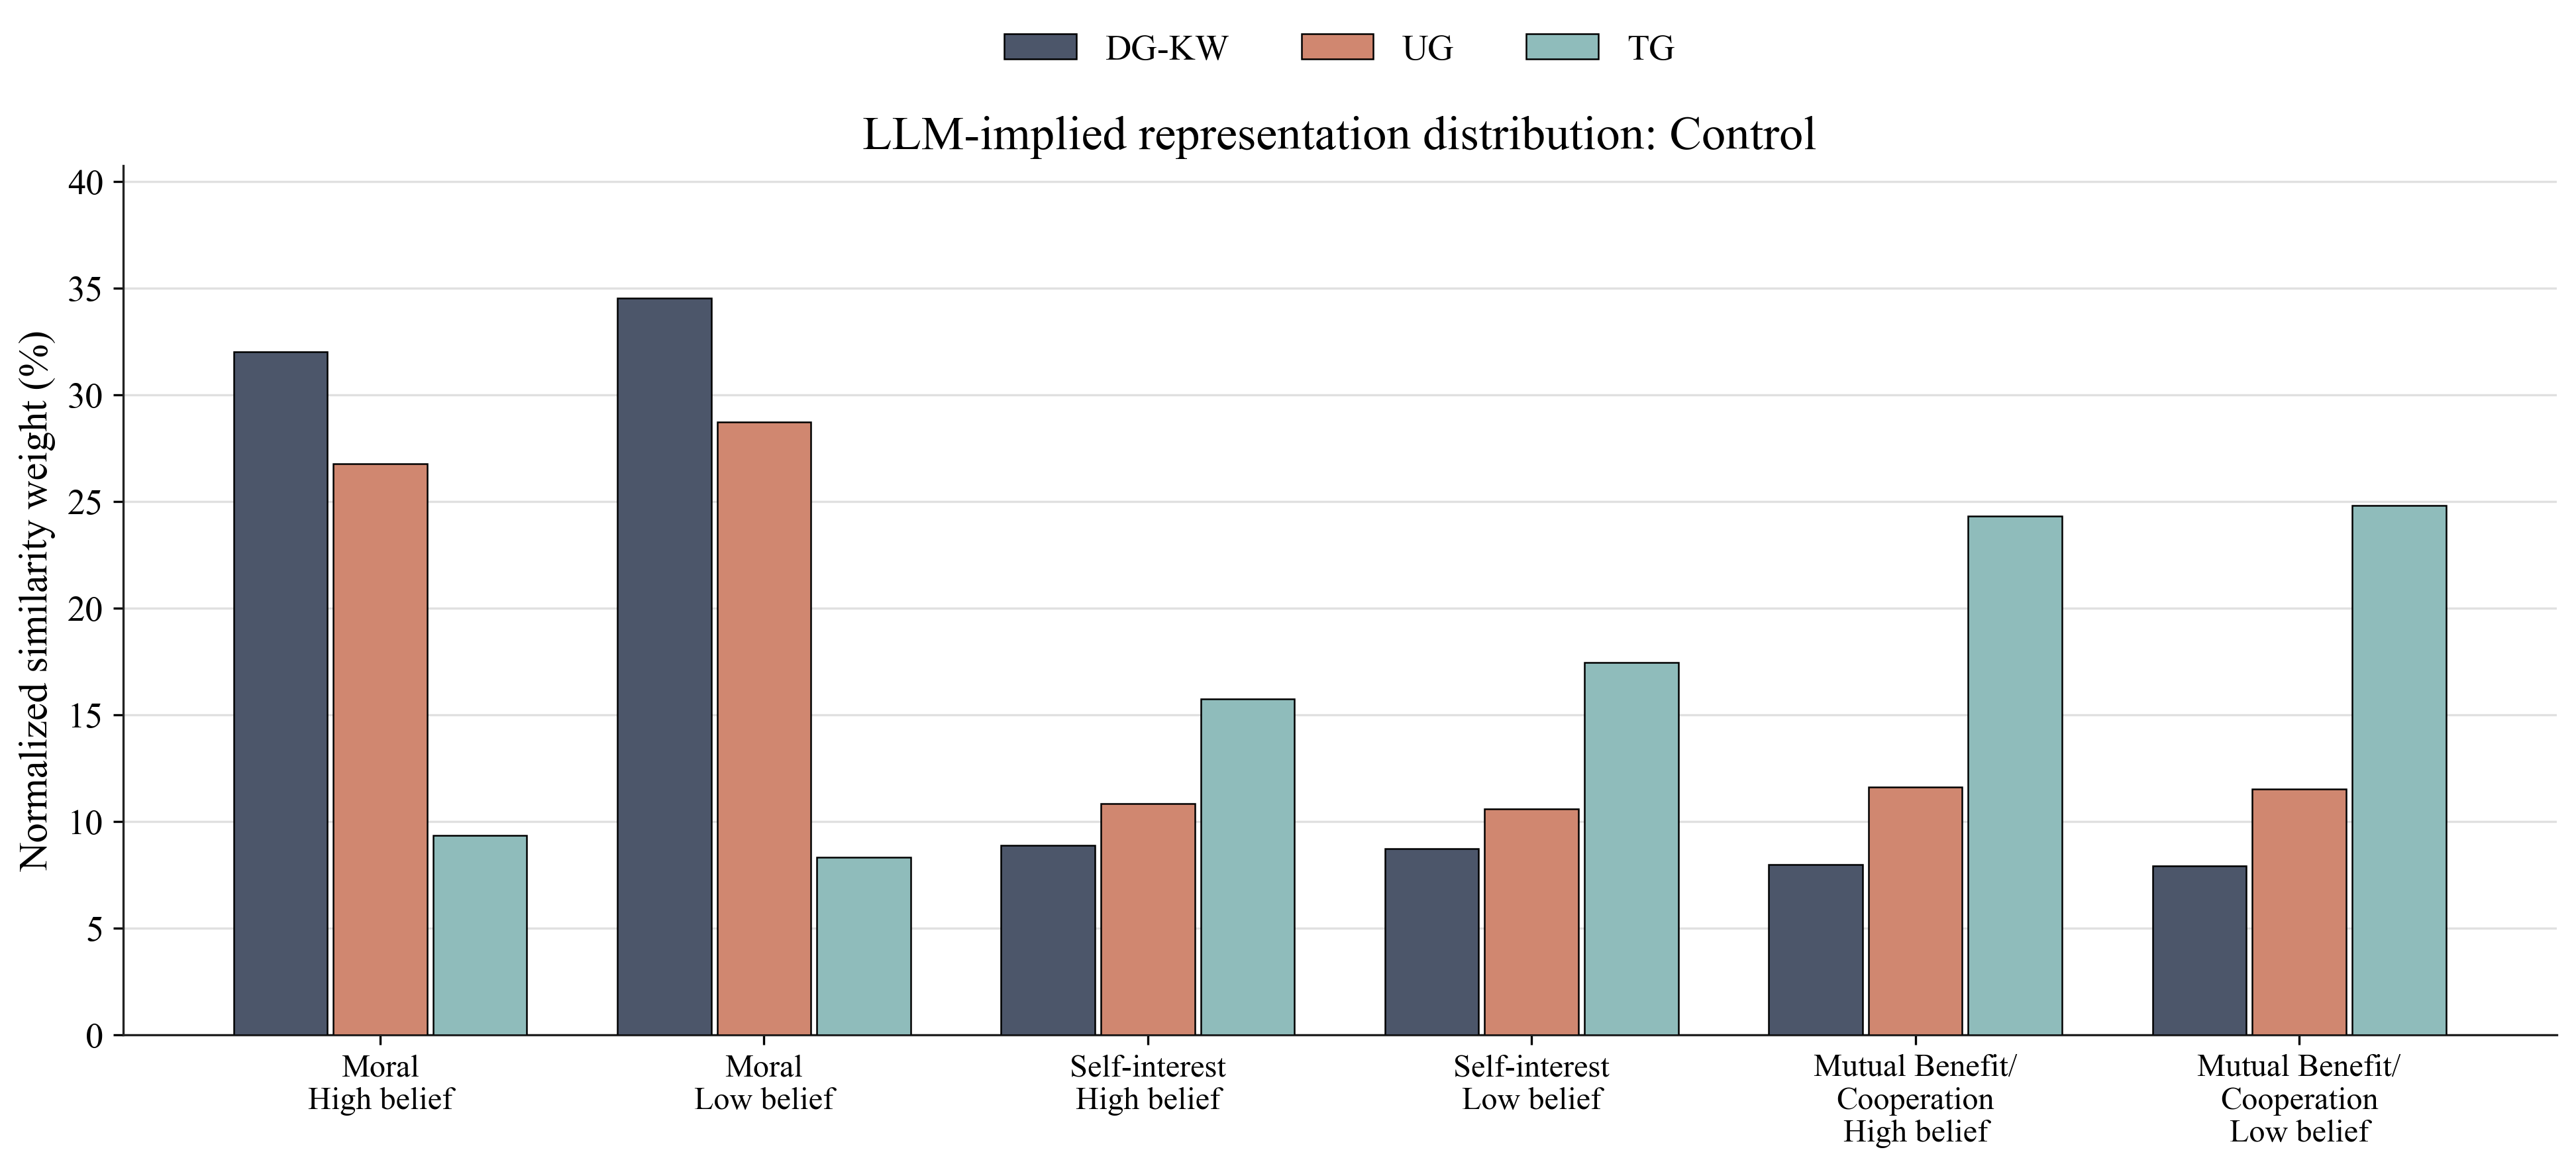
\includegraphics[width=0.95\textwidth]{llm_control_representation_distribution.png}
    \caption{Normalized LLM-implied representation distributions in Control}
    \label{fig:llm_control_representation_distribution}
\end{figure}

\begin{figure}[H]
    \centering
    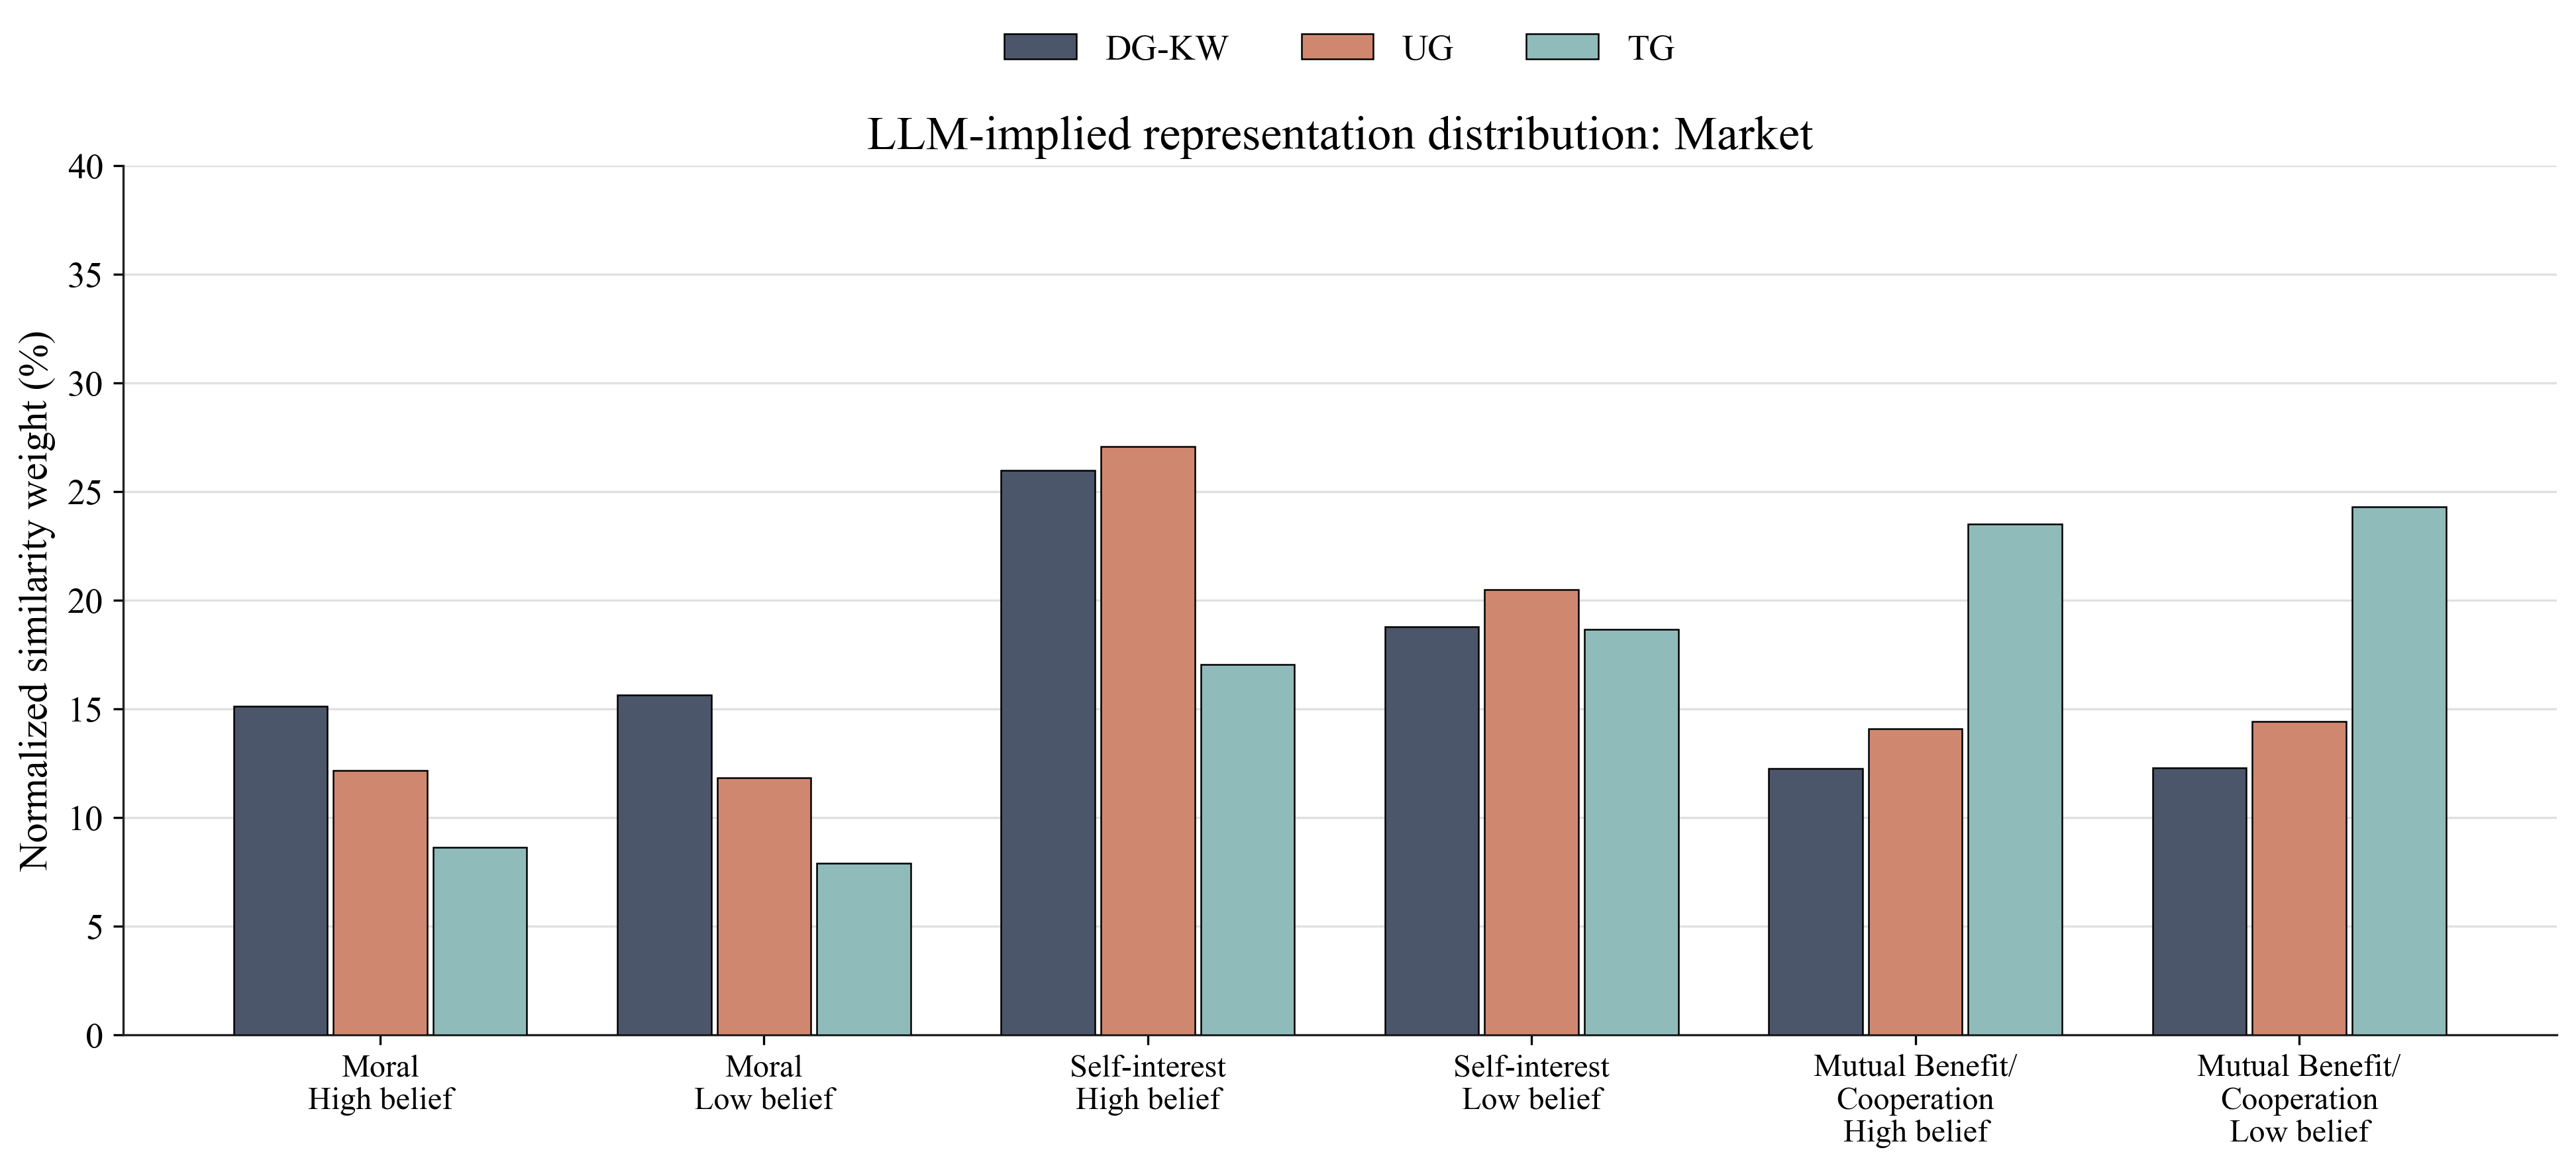
\includegraphics[width=0.95\textwidth]{llm_market_representation_distribution.png}
    \caption{Normalized LLM-implied representation distributions in Market}
    \label{fig:llm_market_representation_distribution}
\end{figure}

\begin{figure}[H]
    \centering
    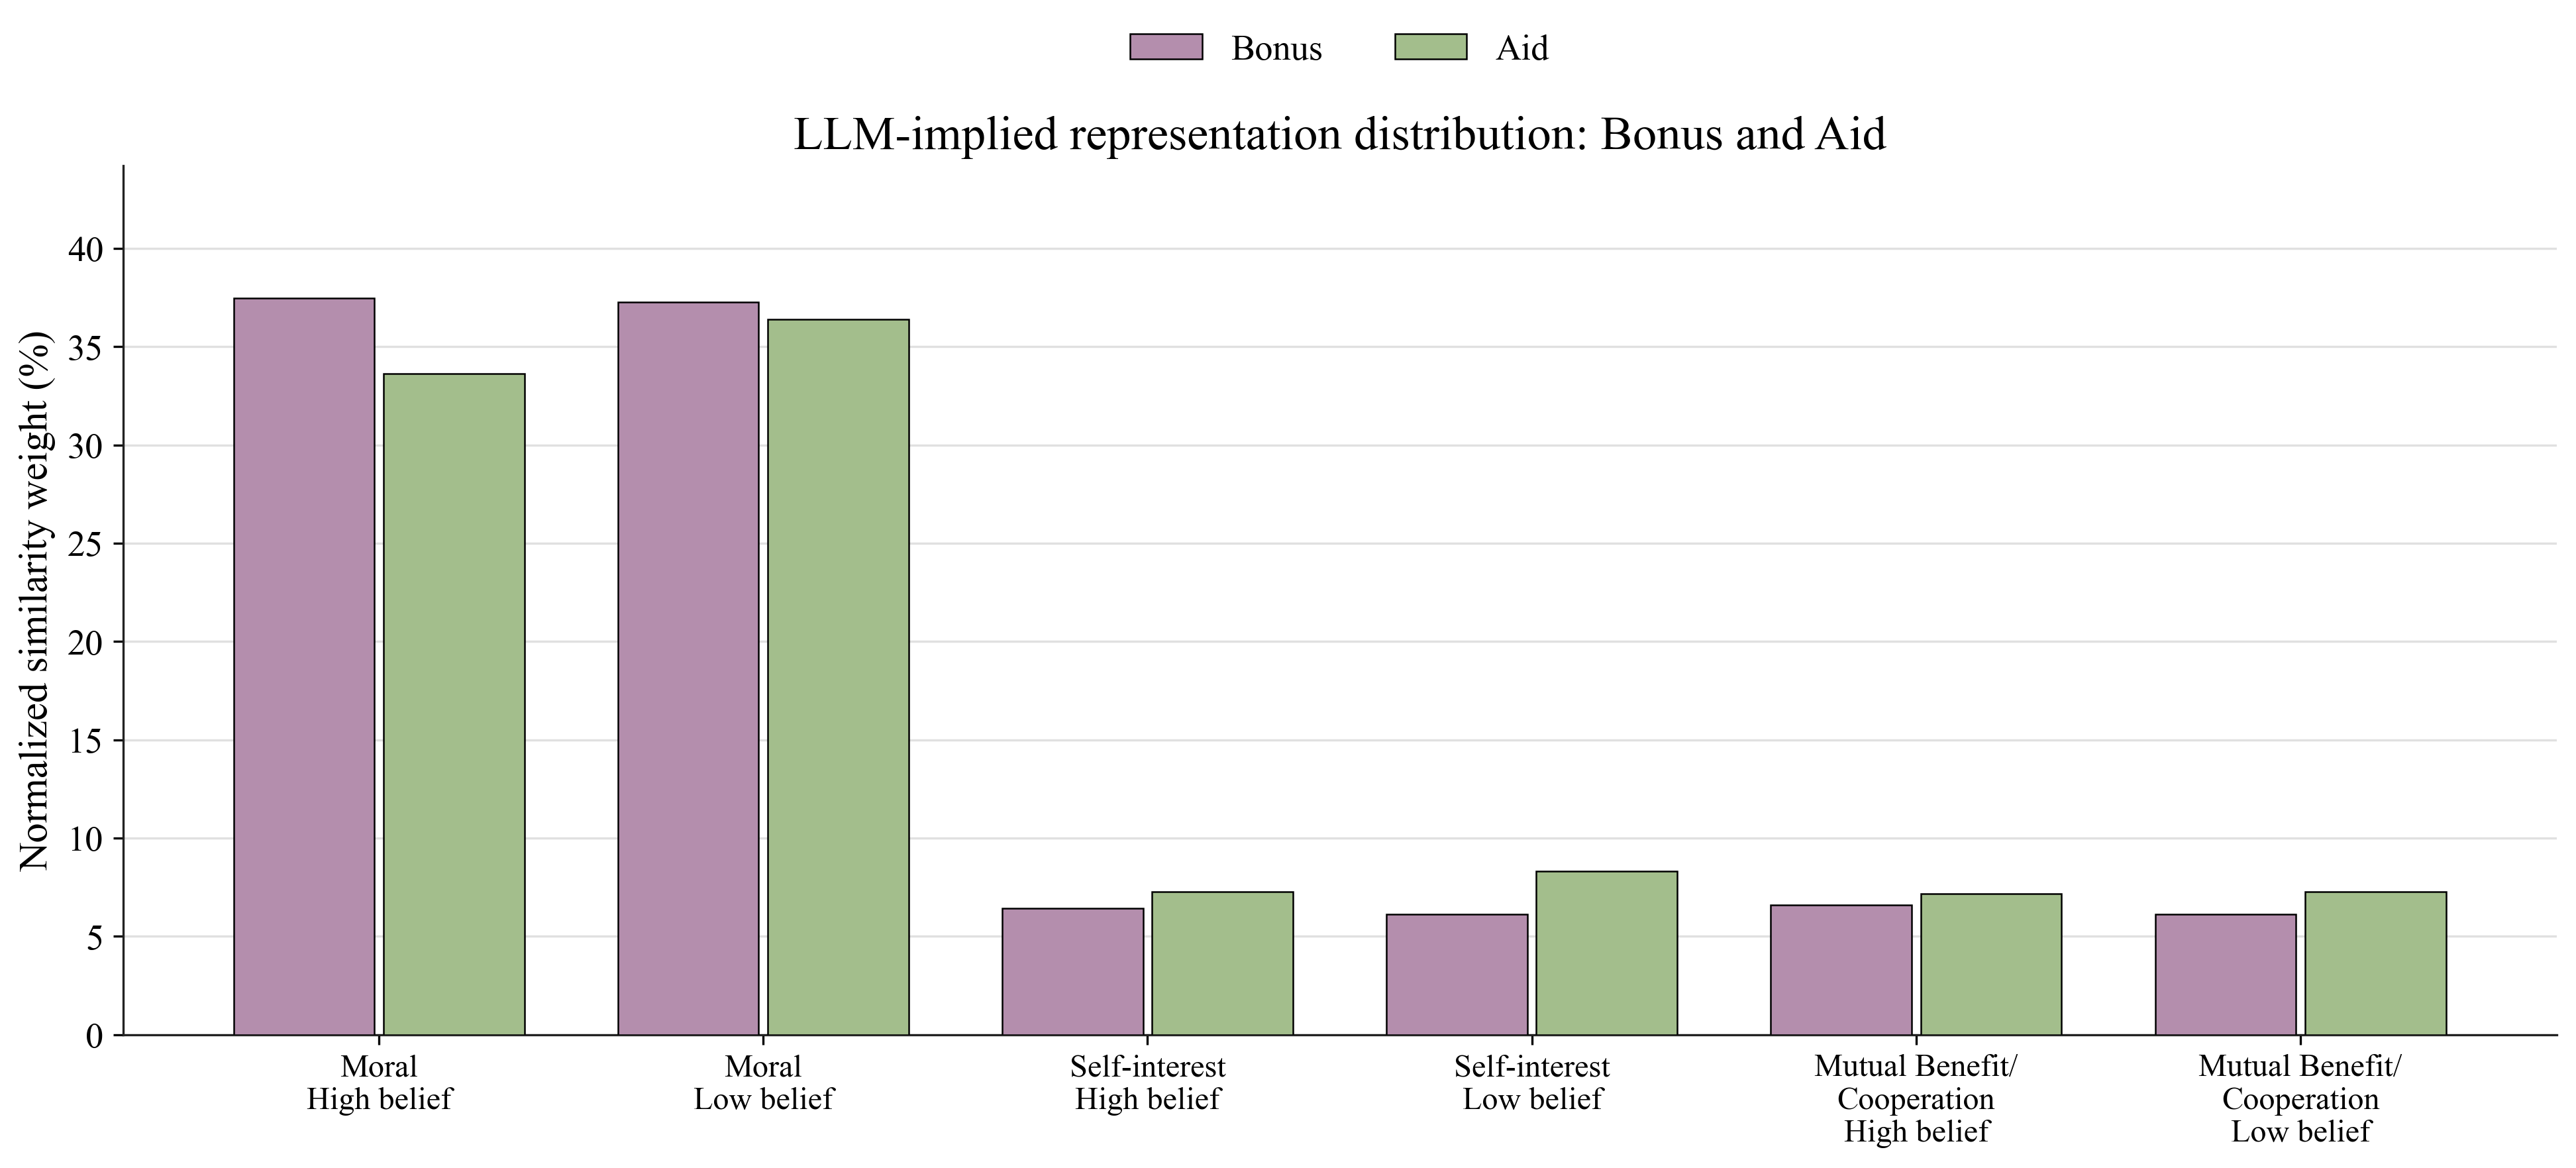
\includegraphics[width=0.95\textwidth]{llm_bonus_aid_representation_distribution.png}
    \caption{Normalized LLM-implied representation distributions in Bonus and Aid}
    \label{fig:llm_bonus_aid_representation_distribution}
\end{figure}

\subsection{Changes Across Conditions}

\begin{figure}[H]
    \centering
    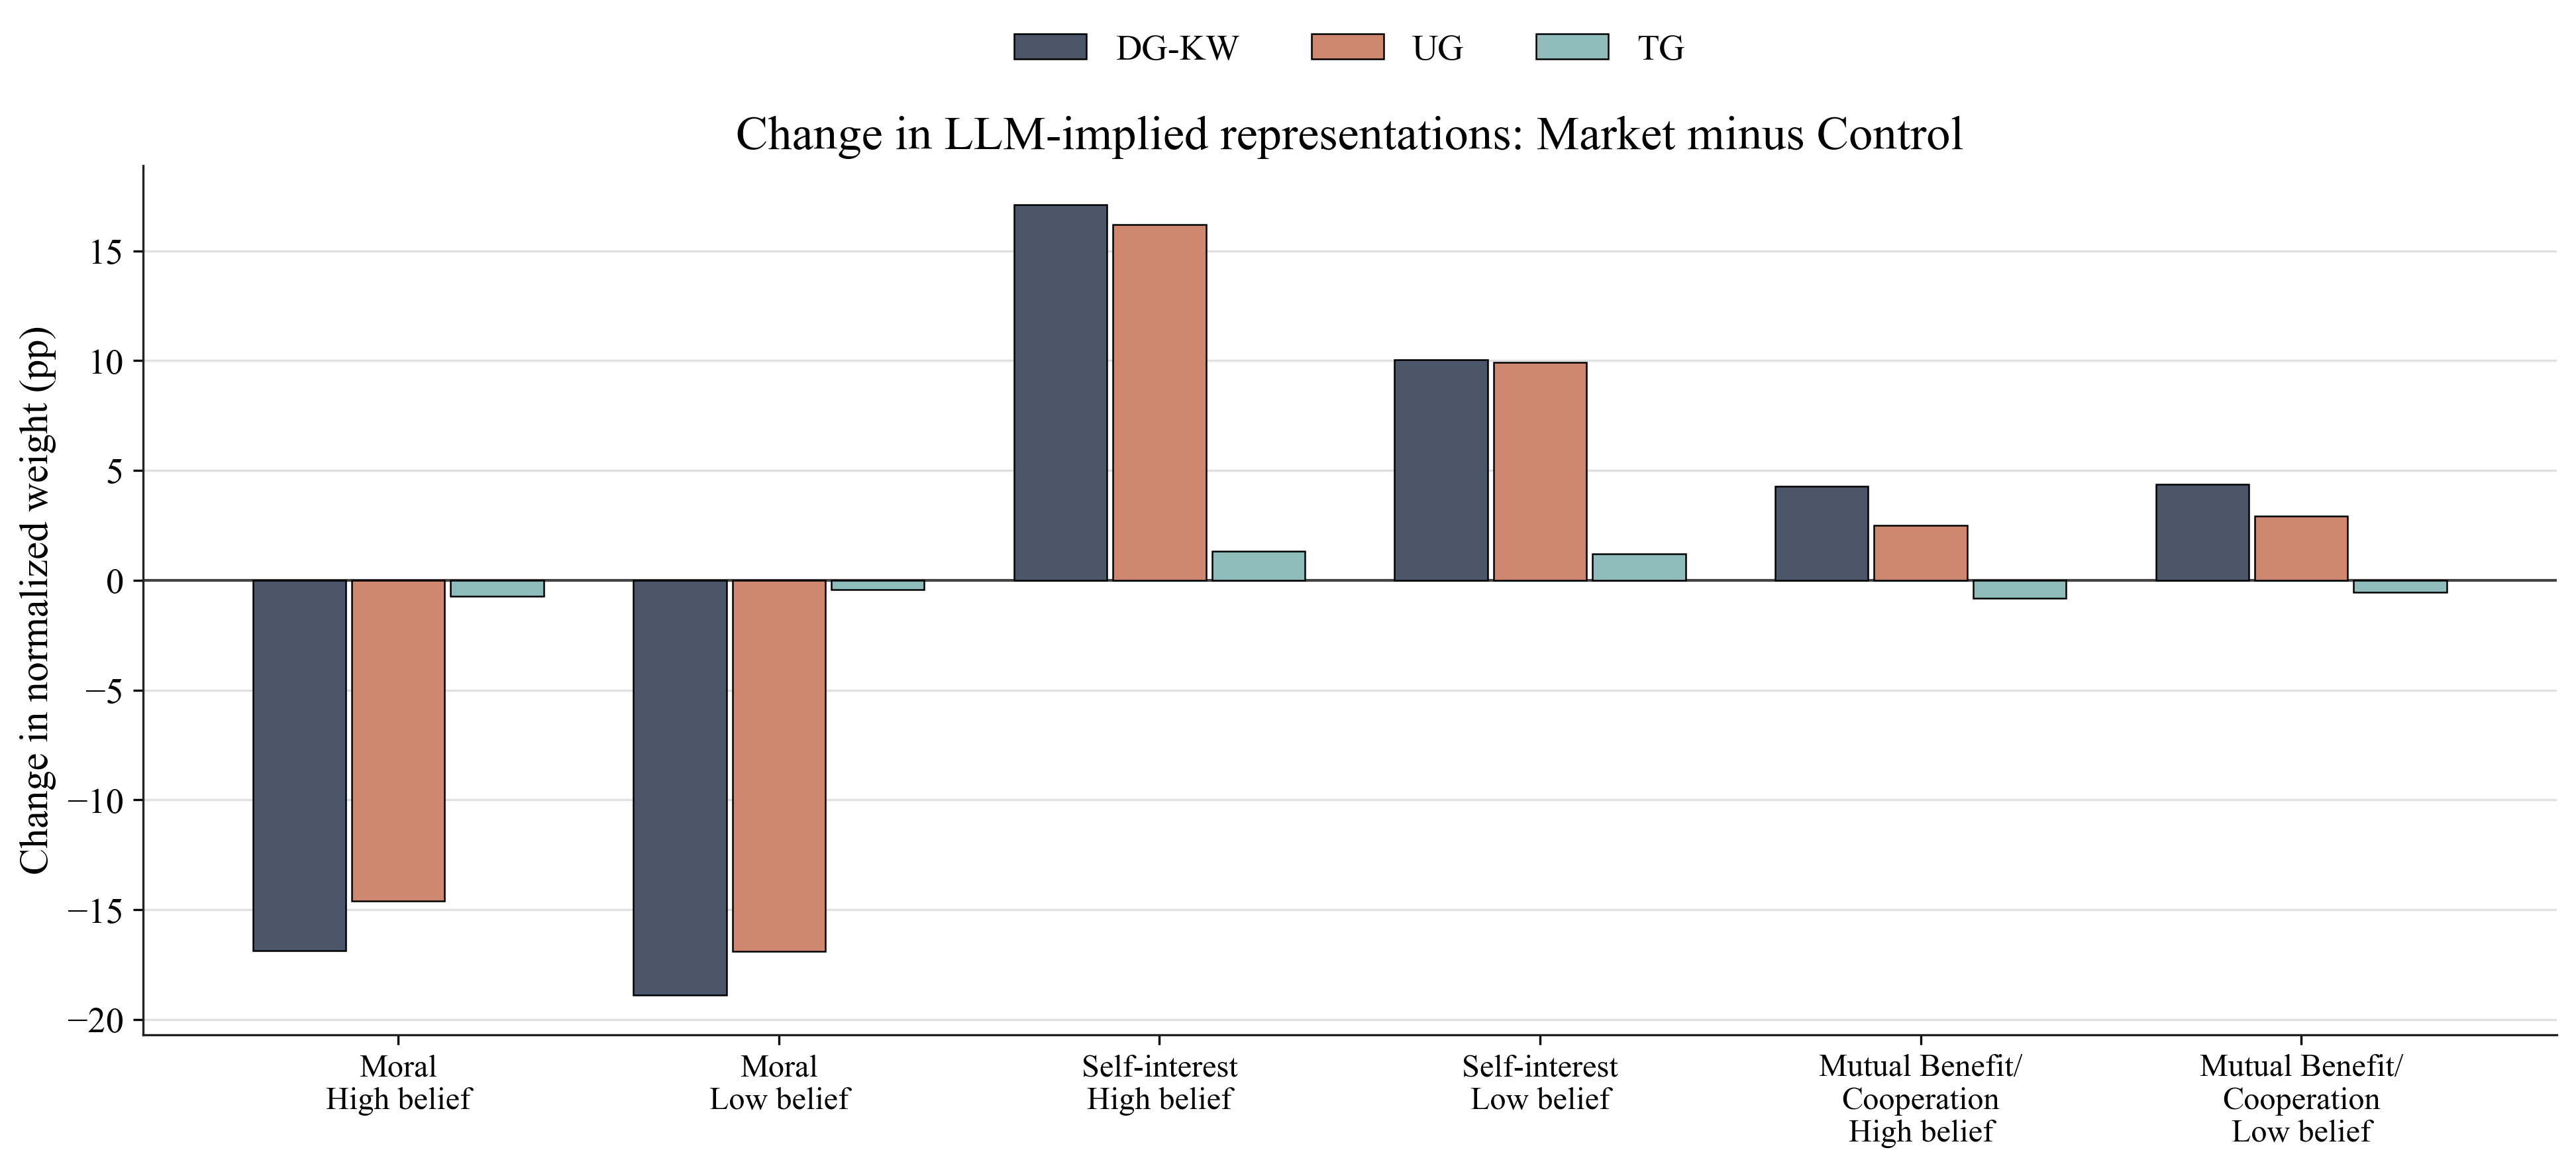
\includegraphics[width=0.95\textwidth]{llm_market_minus_control_representation_difference.png}
    \caption{Change in normalized LLM-implied representation weights: Market minus Control}
    \label{fig:llm_market_minus_control_representation_difference}
\end{figure}

\begin{figure}[H]
    \centering
    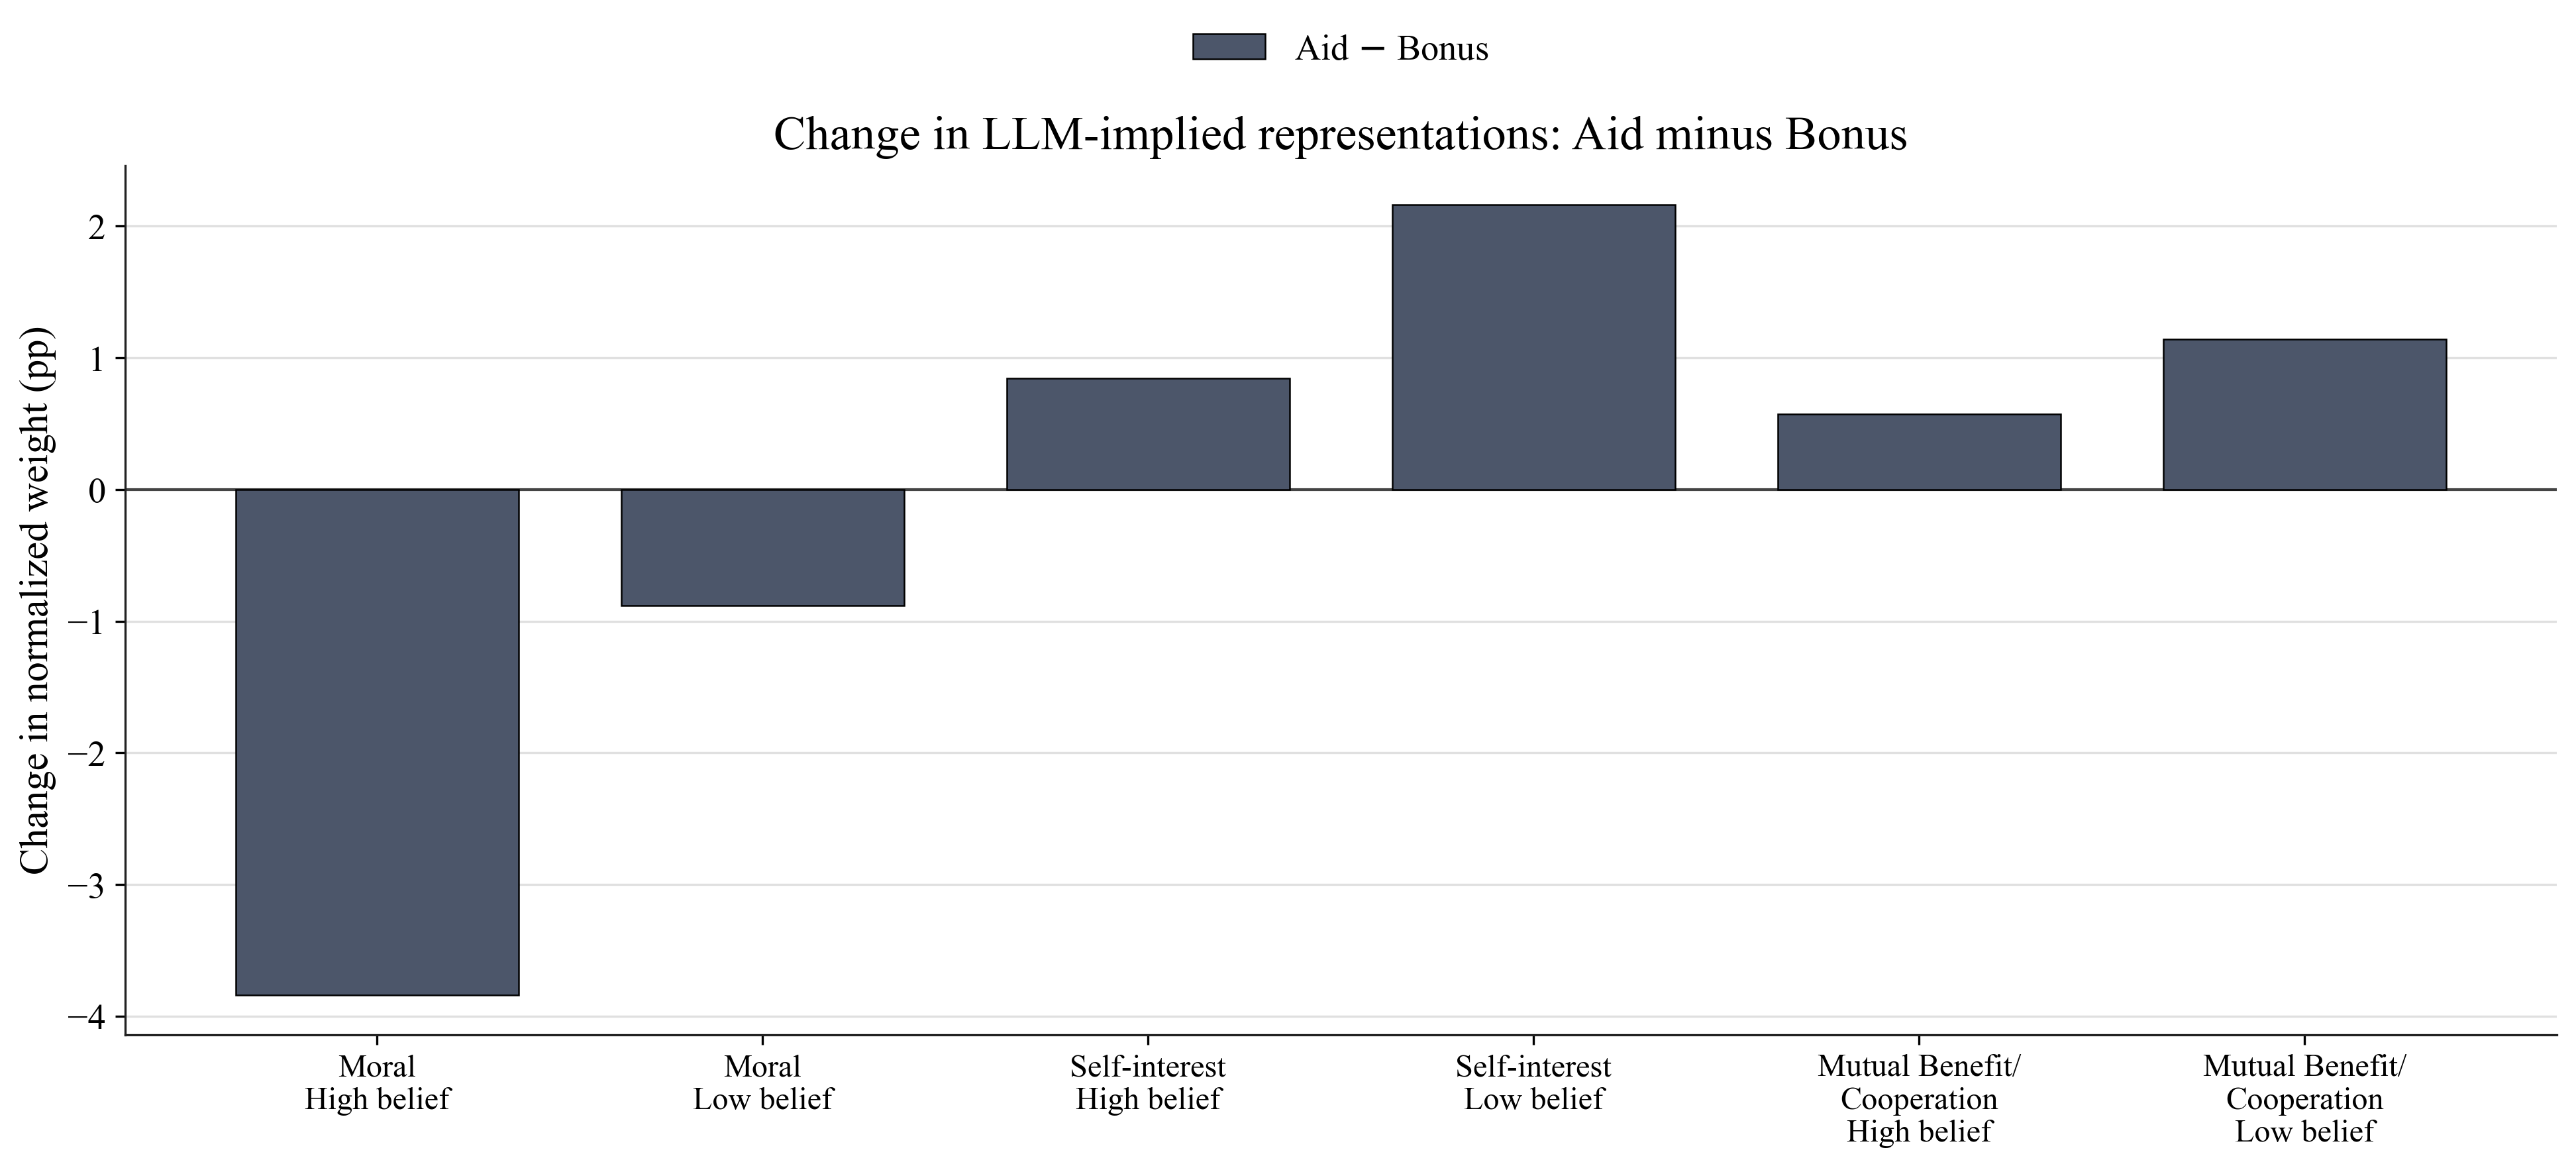
\includegraphics[width=0.95\textwidth]{llm_aid_minus_bonus_representation_difference.png}
    \caption{Change in normalized LLM-implied representation weights: Aid minus Bonus}
    \label{fig:llm_aid_minus_bonus_representation_difference}
\end{figure}

\section{Elicited Representations}

For UG and TG, an elicited representation is the interaction of the classified
reason category and the participant's hypothetical belief. The High/Low cutoff
is calculated separately within each game and comparison, pooling Control with
Market for their comparison and Bonus with Aid for theirs. High denotes a belief
strictly above the pooled median; observations at the median are assigned to Low,
so identical belief values are not split across groups. The figures use classified
participants with non-missing hypothetical beliefs. Consequently, each condition's
six displayed shares sum to 100, but sample sizes can differ across conditions.

DG-KW has no elicited belief. It therefore cannot be divided into the six cells
without imposing an artificial belief classification; its three reason-category
shares are reported separately in Section~\ref{sec:dg_categories}.

\subsection{Levels}

\begin{figure}[H]
    \centering
    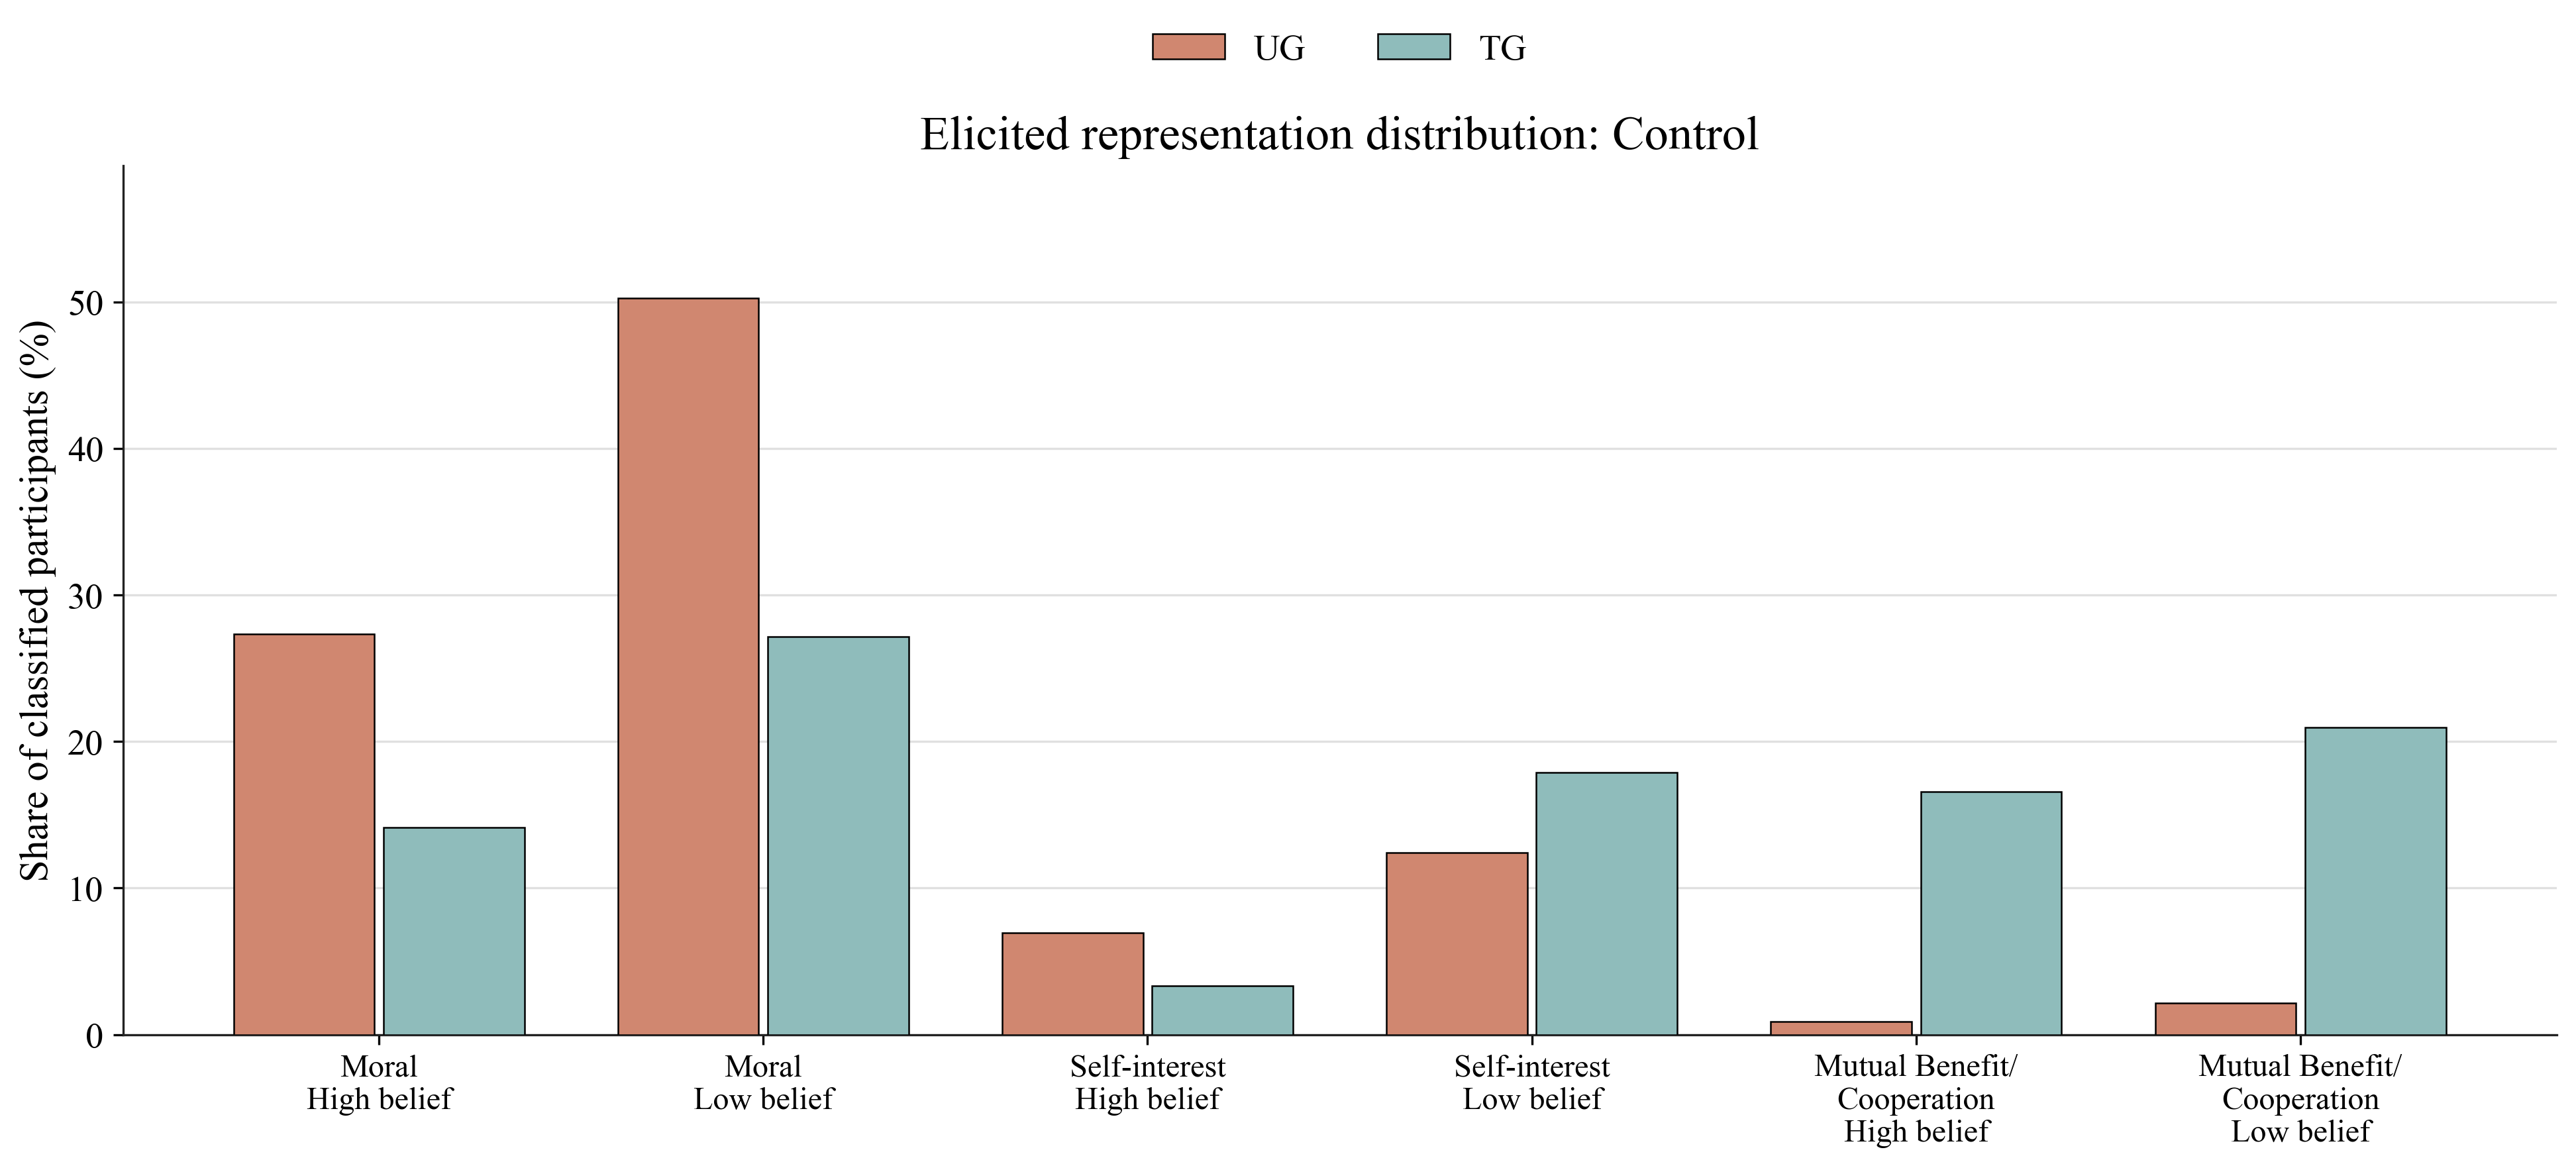
\includegraphics[width=0.95\textwidth]{elicited_control_representation_distribution.png}
    \caption{Elicited representation distributions in Control}
    \label{fig:elicited_control_representation_distribution}
\end{figure}

\begin{figure}[H]
    \centering
    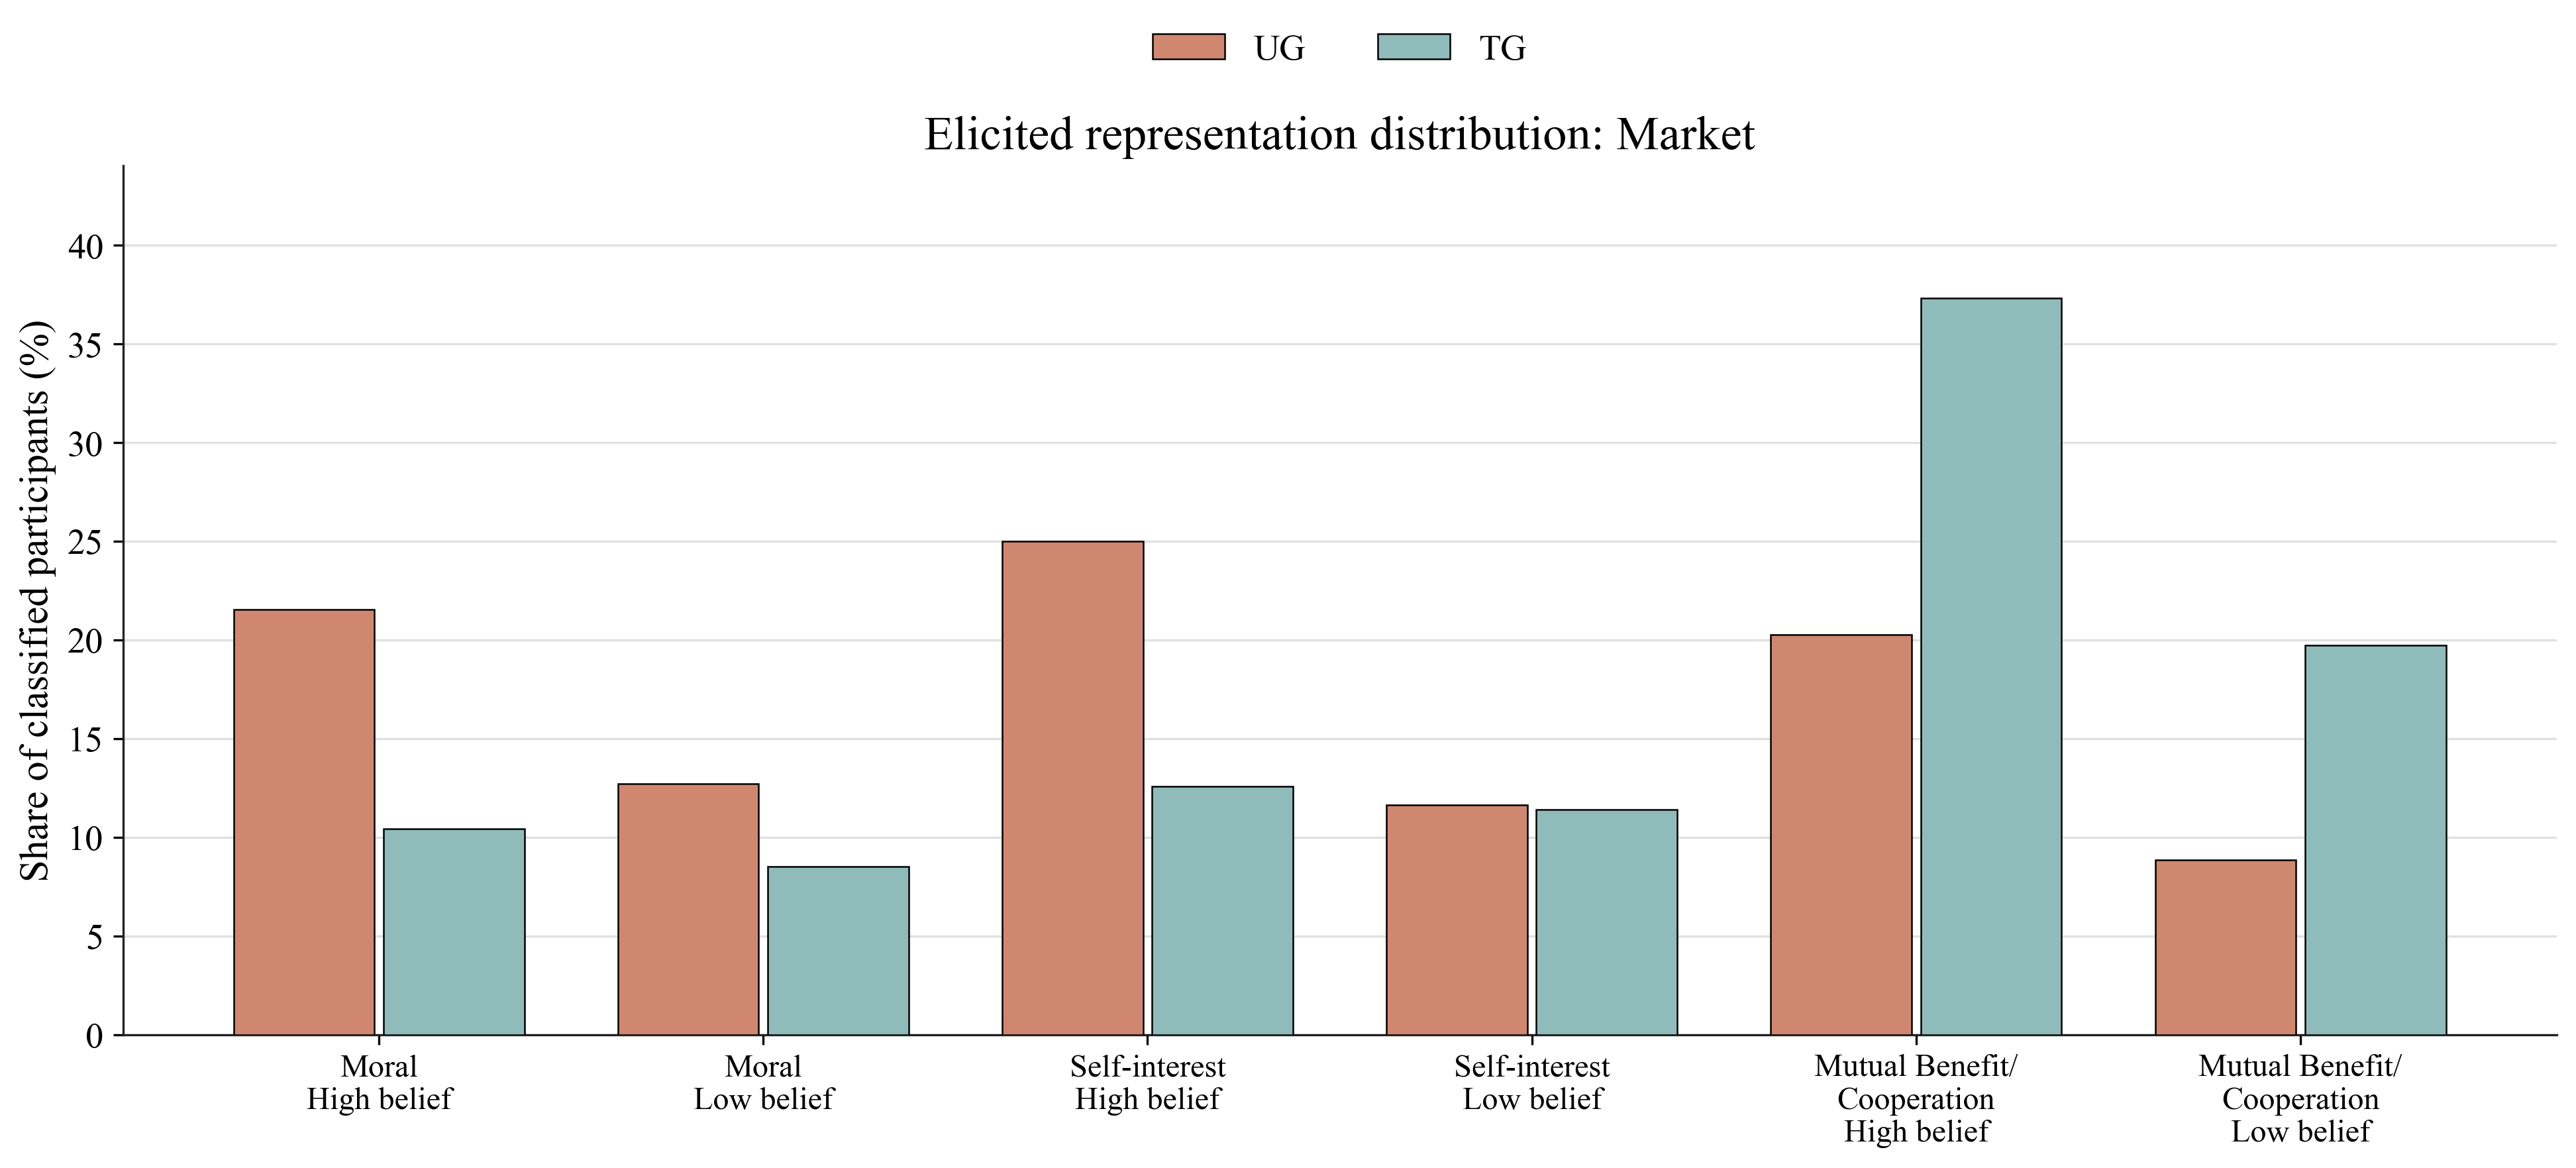
\includegraphics[width=0.95\textwidth]{elicited_market_representation_distribution.png}
    \caption{Elicited representation distributions in Market}
    \label{fig:elicited_market_representation_distribution}
\end{figure}

\begin{figure}[H]
    \centering
    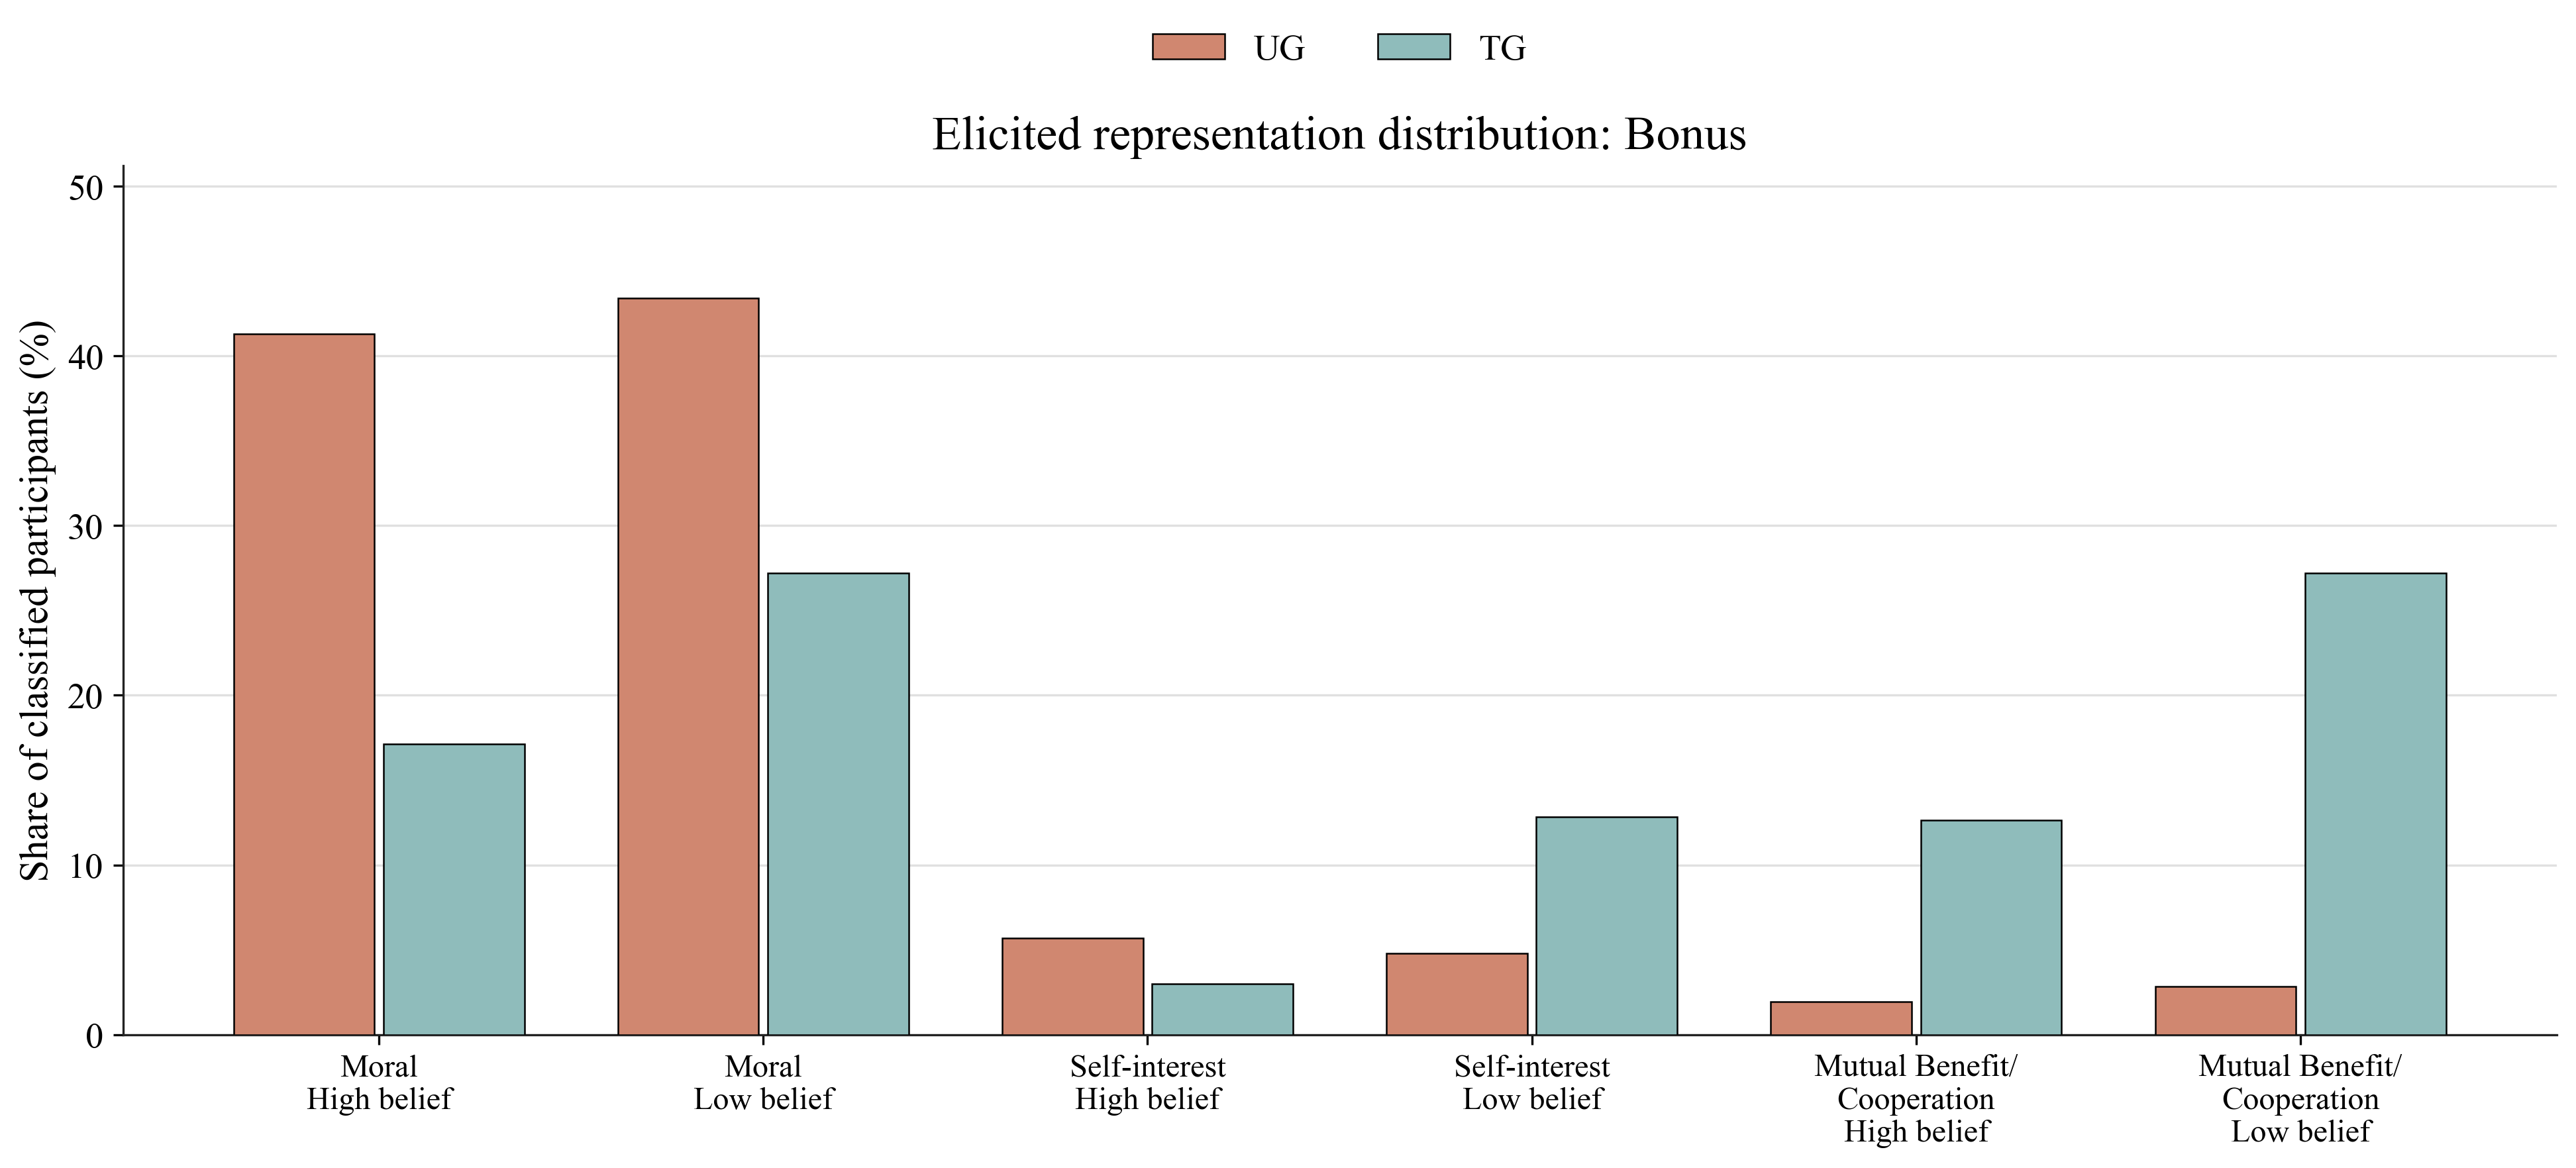
\includegraphics[width=0.95\textwidth]{elicited_bonus_representation_distribution.png}
    \caption{Elicited representation distributions in Bonus}
    \label{fig:elicited_bonus_representation_distribution}
\end{figure}

\begin{figure}[H]
    \centering
    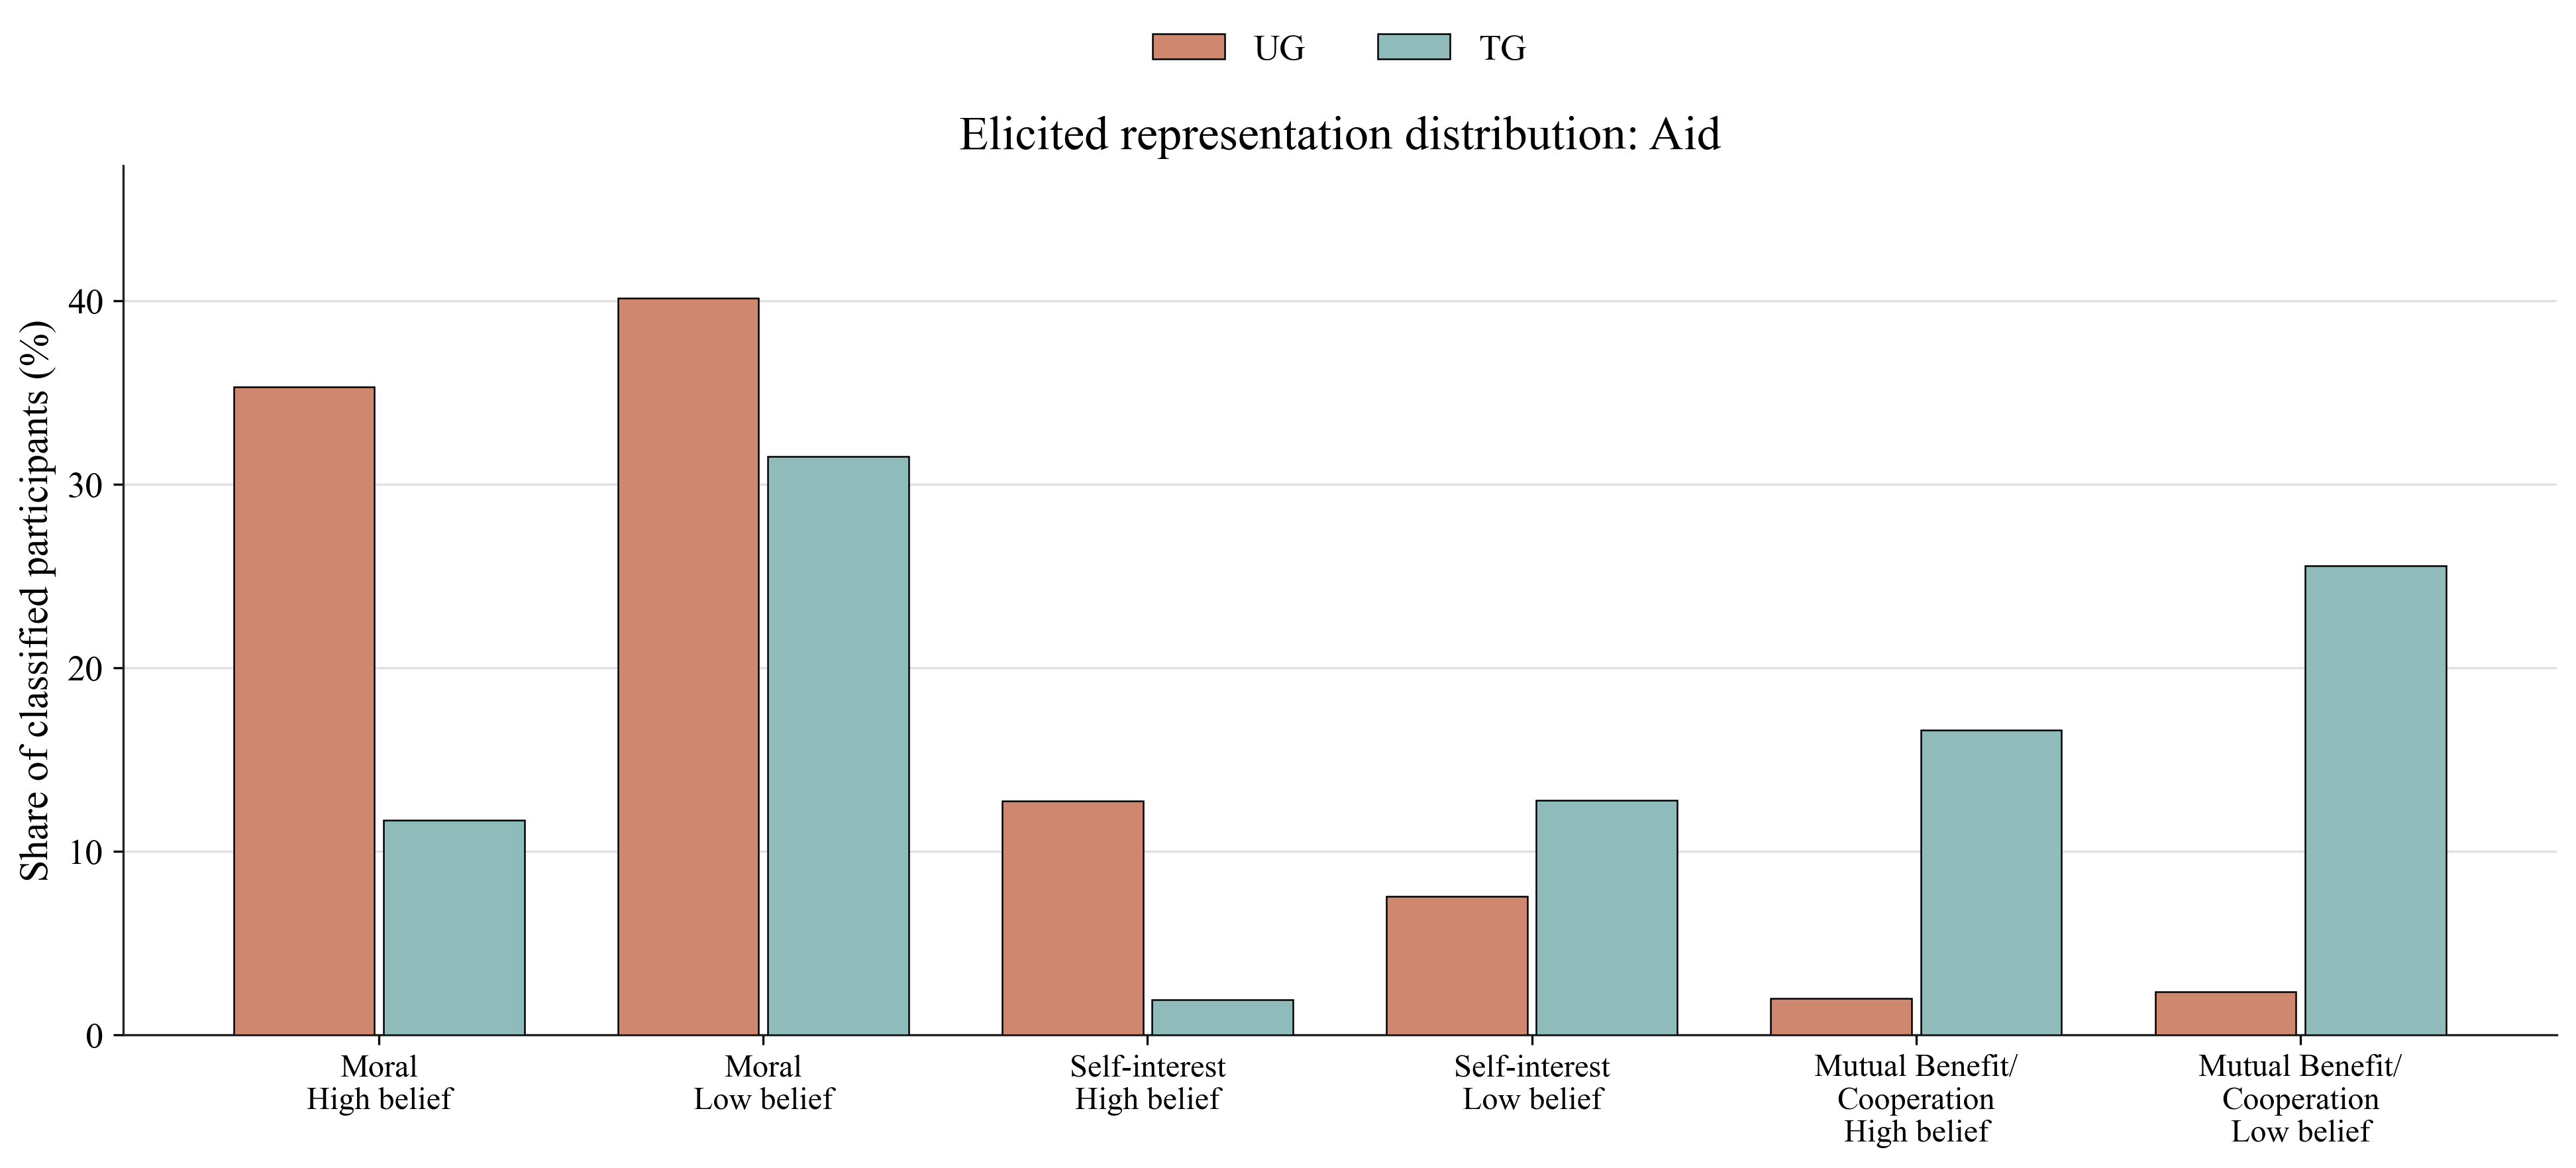
\includegraphics[width=0.95\textwidth]{elicited_aid_representation_distribution.png}
    \caption{Elicited representation distributions in Aid}
    \label{fig:elicited_aid_representation_distribution}
\end{figure}

\subsection{Changes Across Conditions}

\begin{figure}[H]
    \centering
    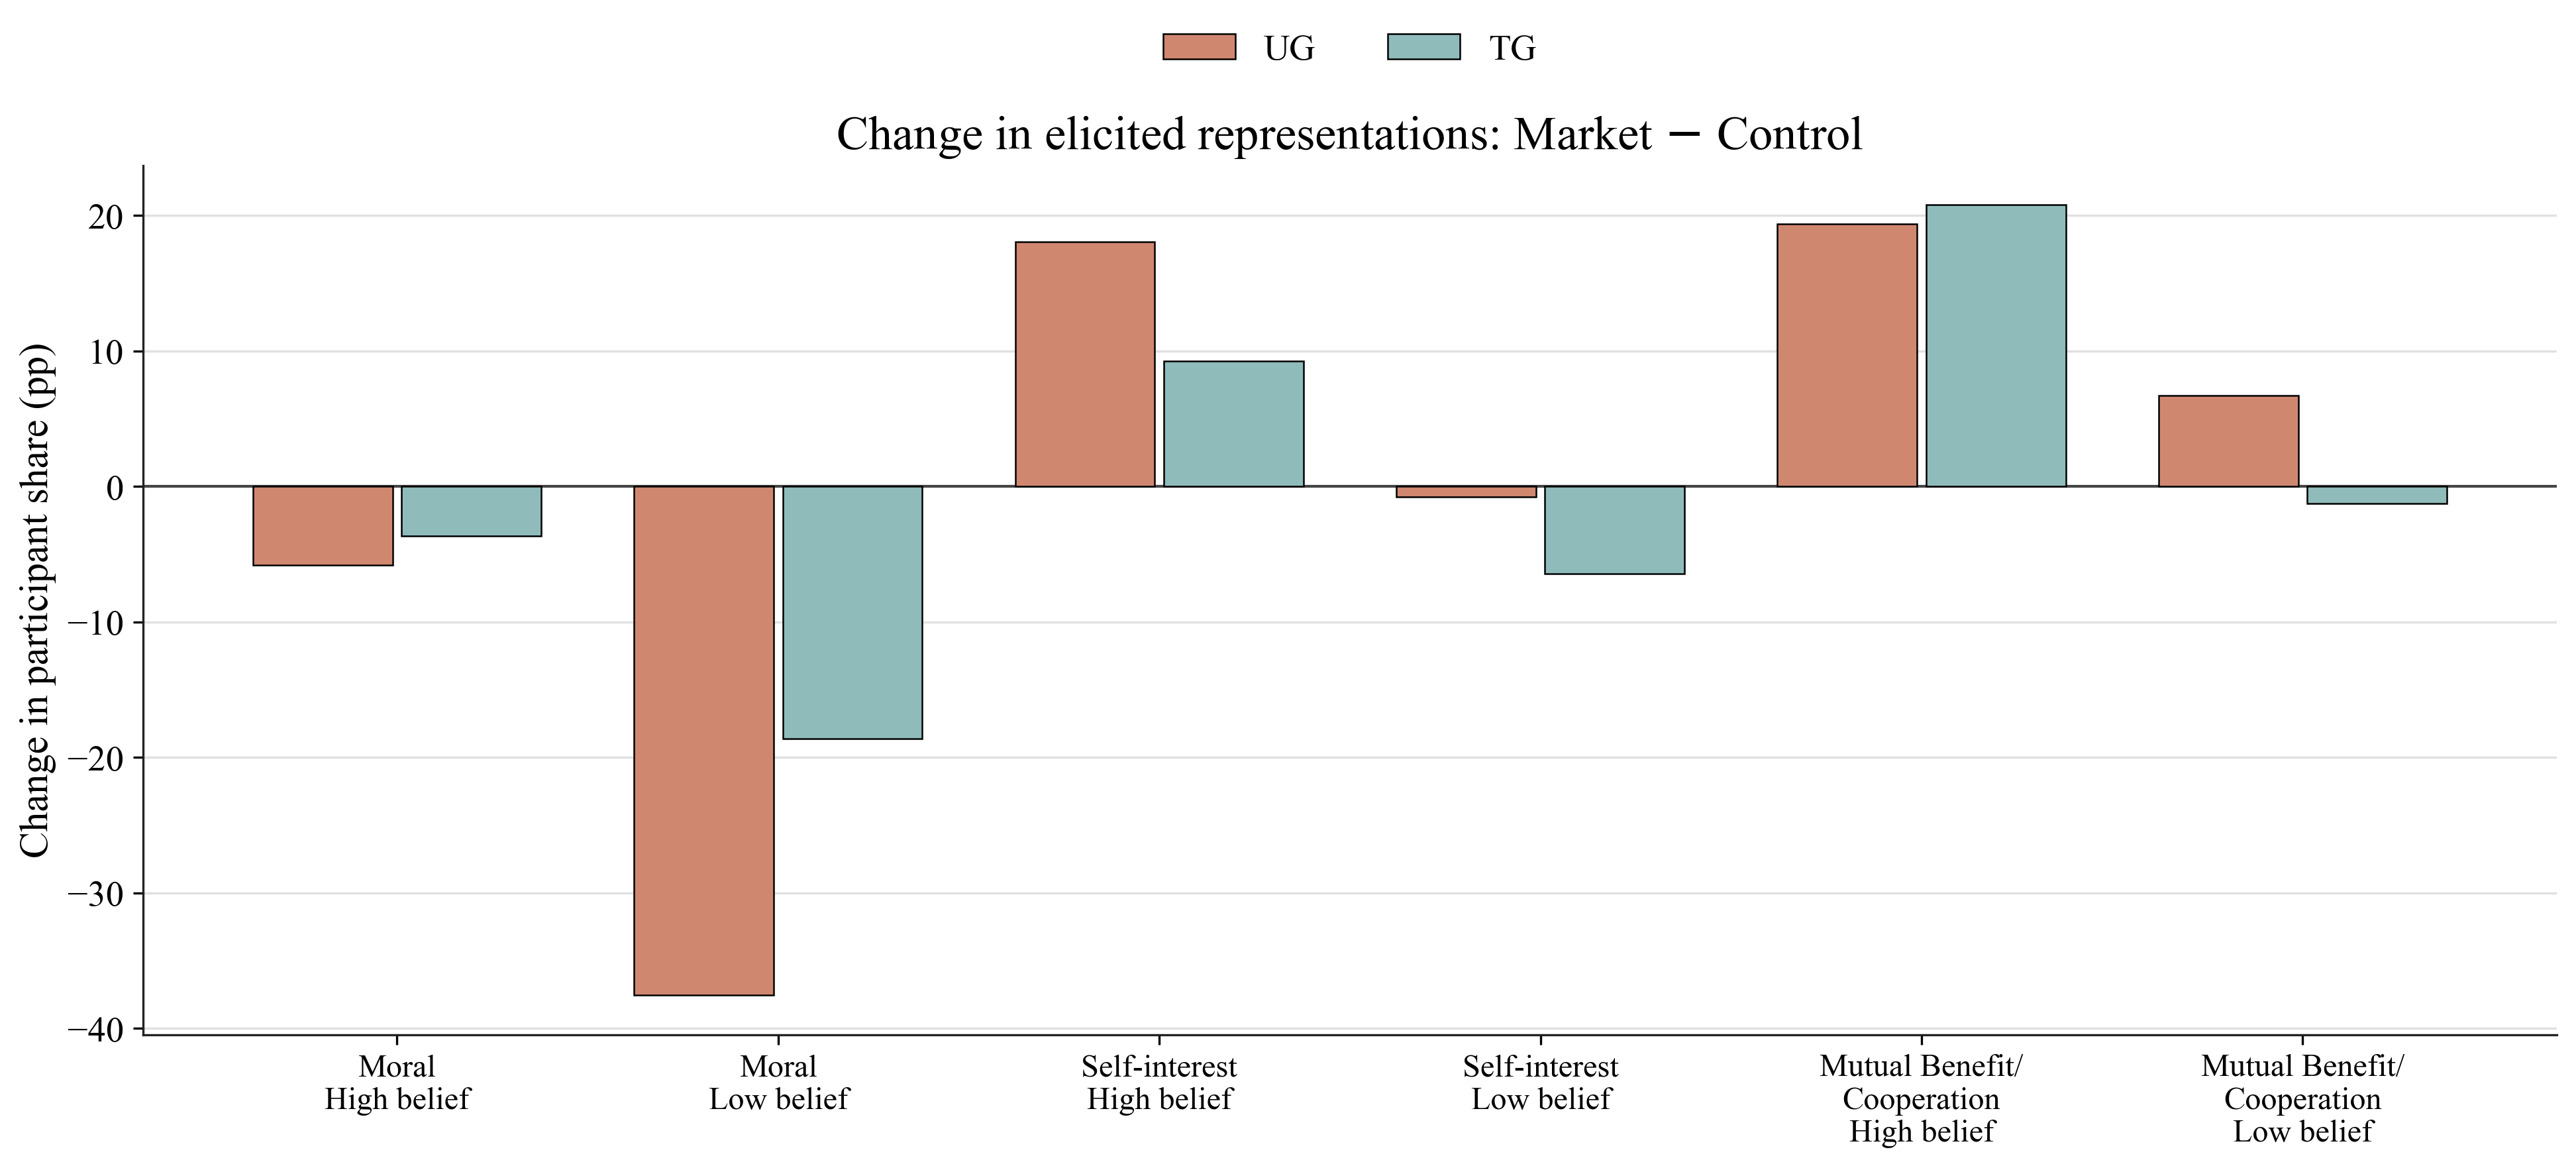
\includegraphics[width=0.95\textwidth]{elicited_market_vs_control_representation_difference.png}
    \caption{Change in elicited representation shares: Market minus Control}
    \label{fig:elicited_market_vs_control_representation_difference}
\end{figure}

\begin{figure}[H]
    \centering
    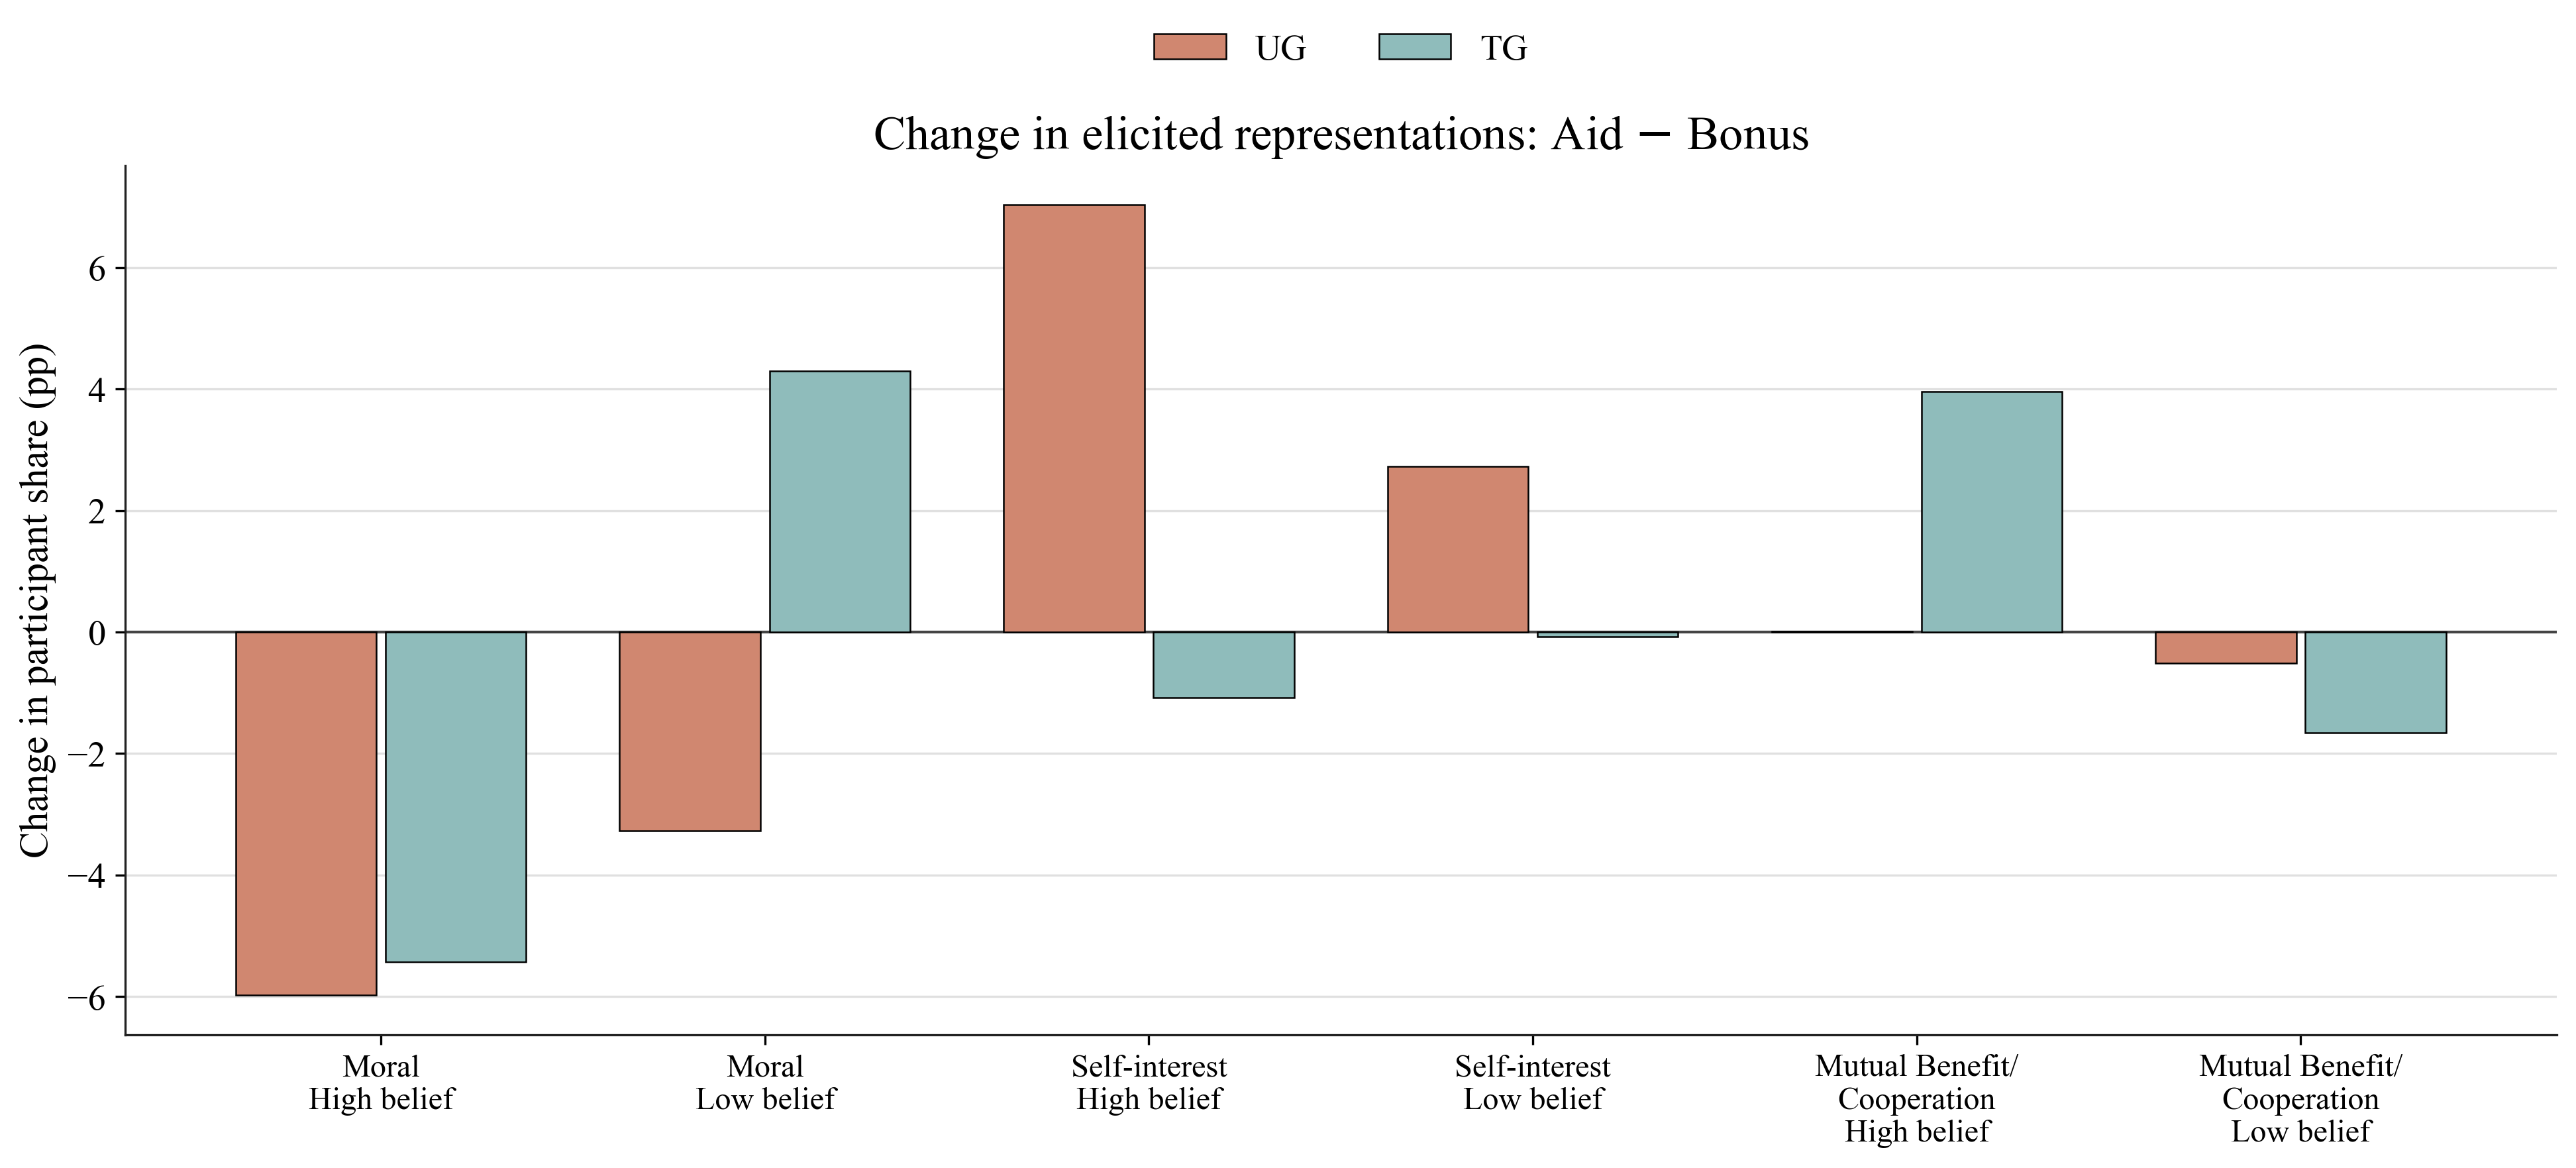
\includegraphics[width=0.95\textwidth]{elicited_aid_vs_bonus_representation_difference.png}
    \caption{Change in elicited representation shares: Aid minus Bonus}
    \label{fig:elicited_aid_vs_bonus_representation_difference}
\end{figure}

\section{DG-KW Elicited Reason Categories}
\label{sec:dg_categories}

\begin{figure}[H]
    \centering
    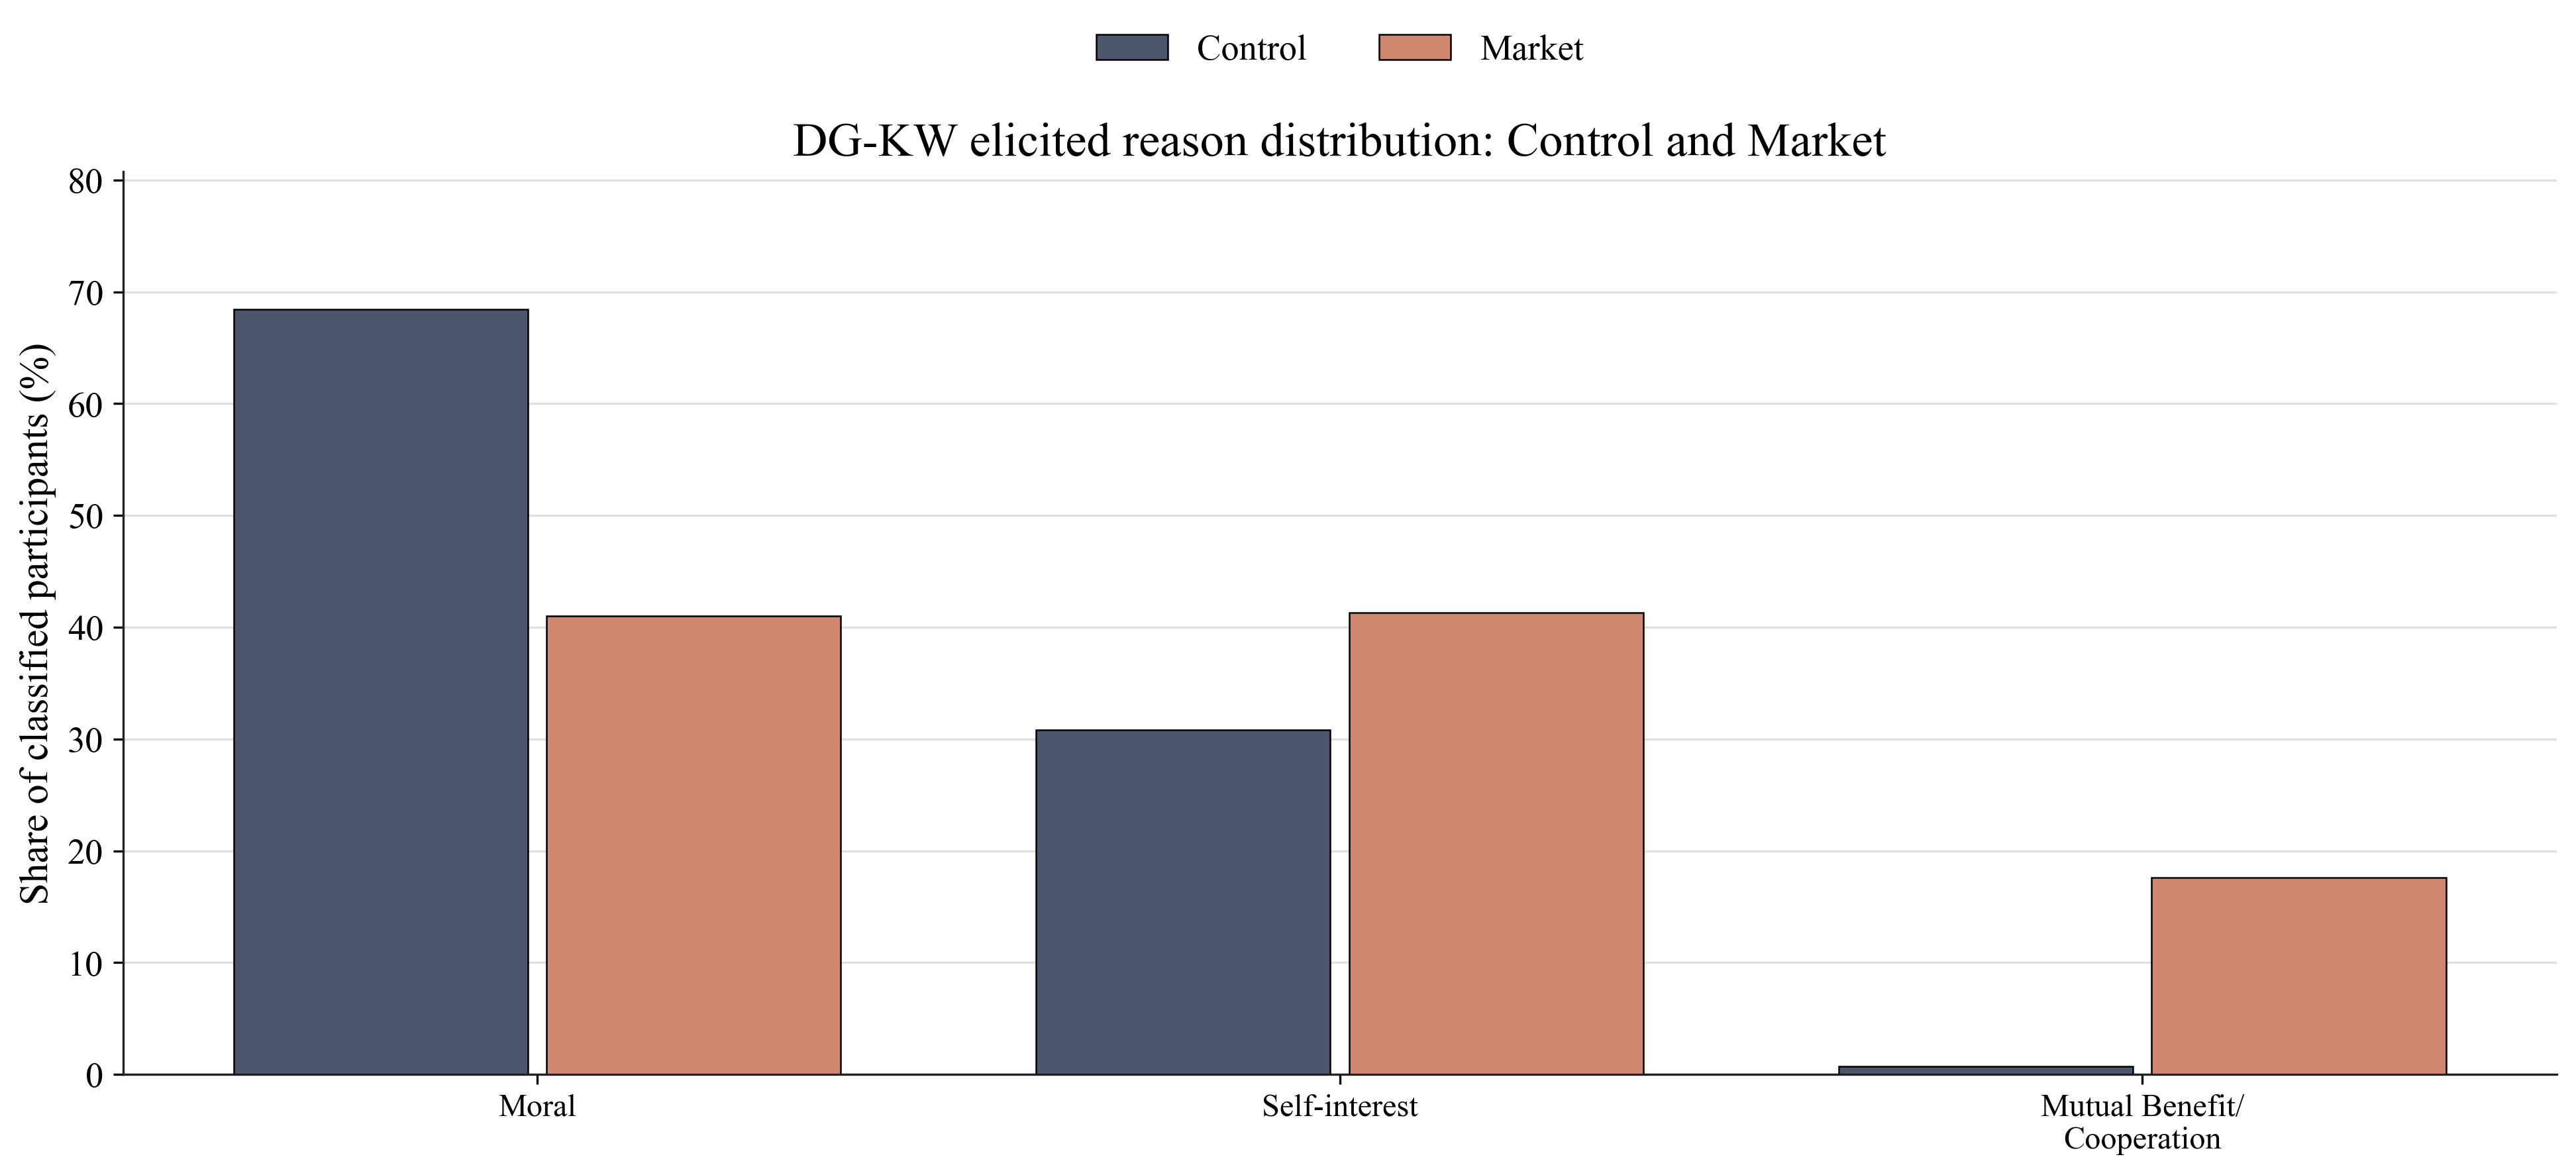
\includegraphics[width=0.95\textwidth]{elicited_dg_control_market_category_distribution.png}
    \caption{DG-KW elicited reason-category distributions in Control and Market}
    \label{fig:elicited_dg_control_market_category_distributions}
\end{figure}

\begin{figure}[H]
    \centering
    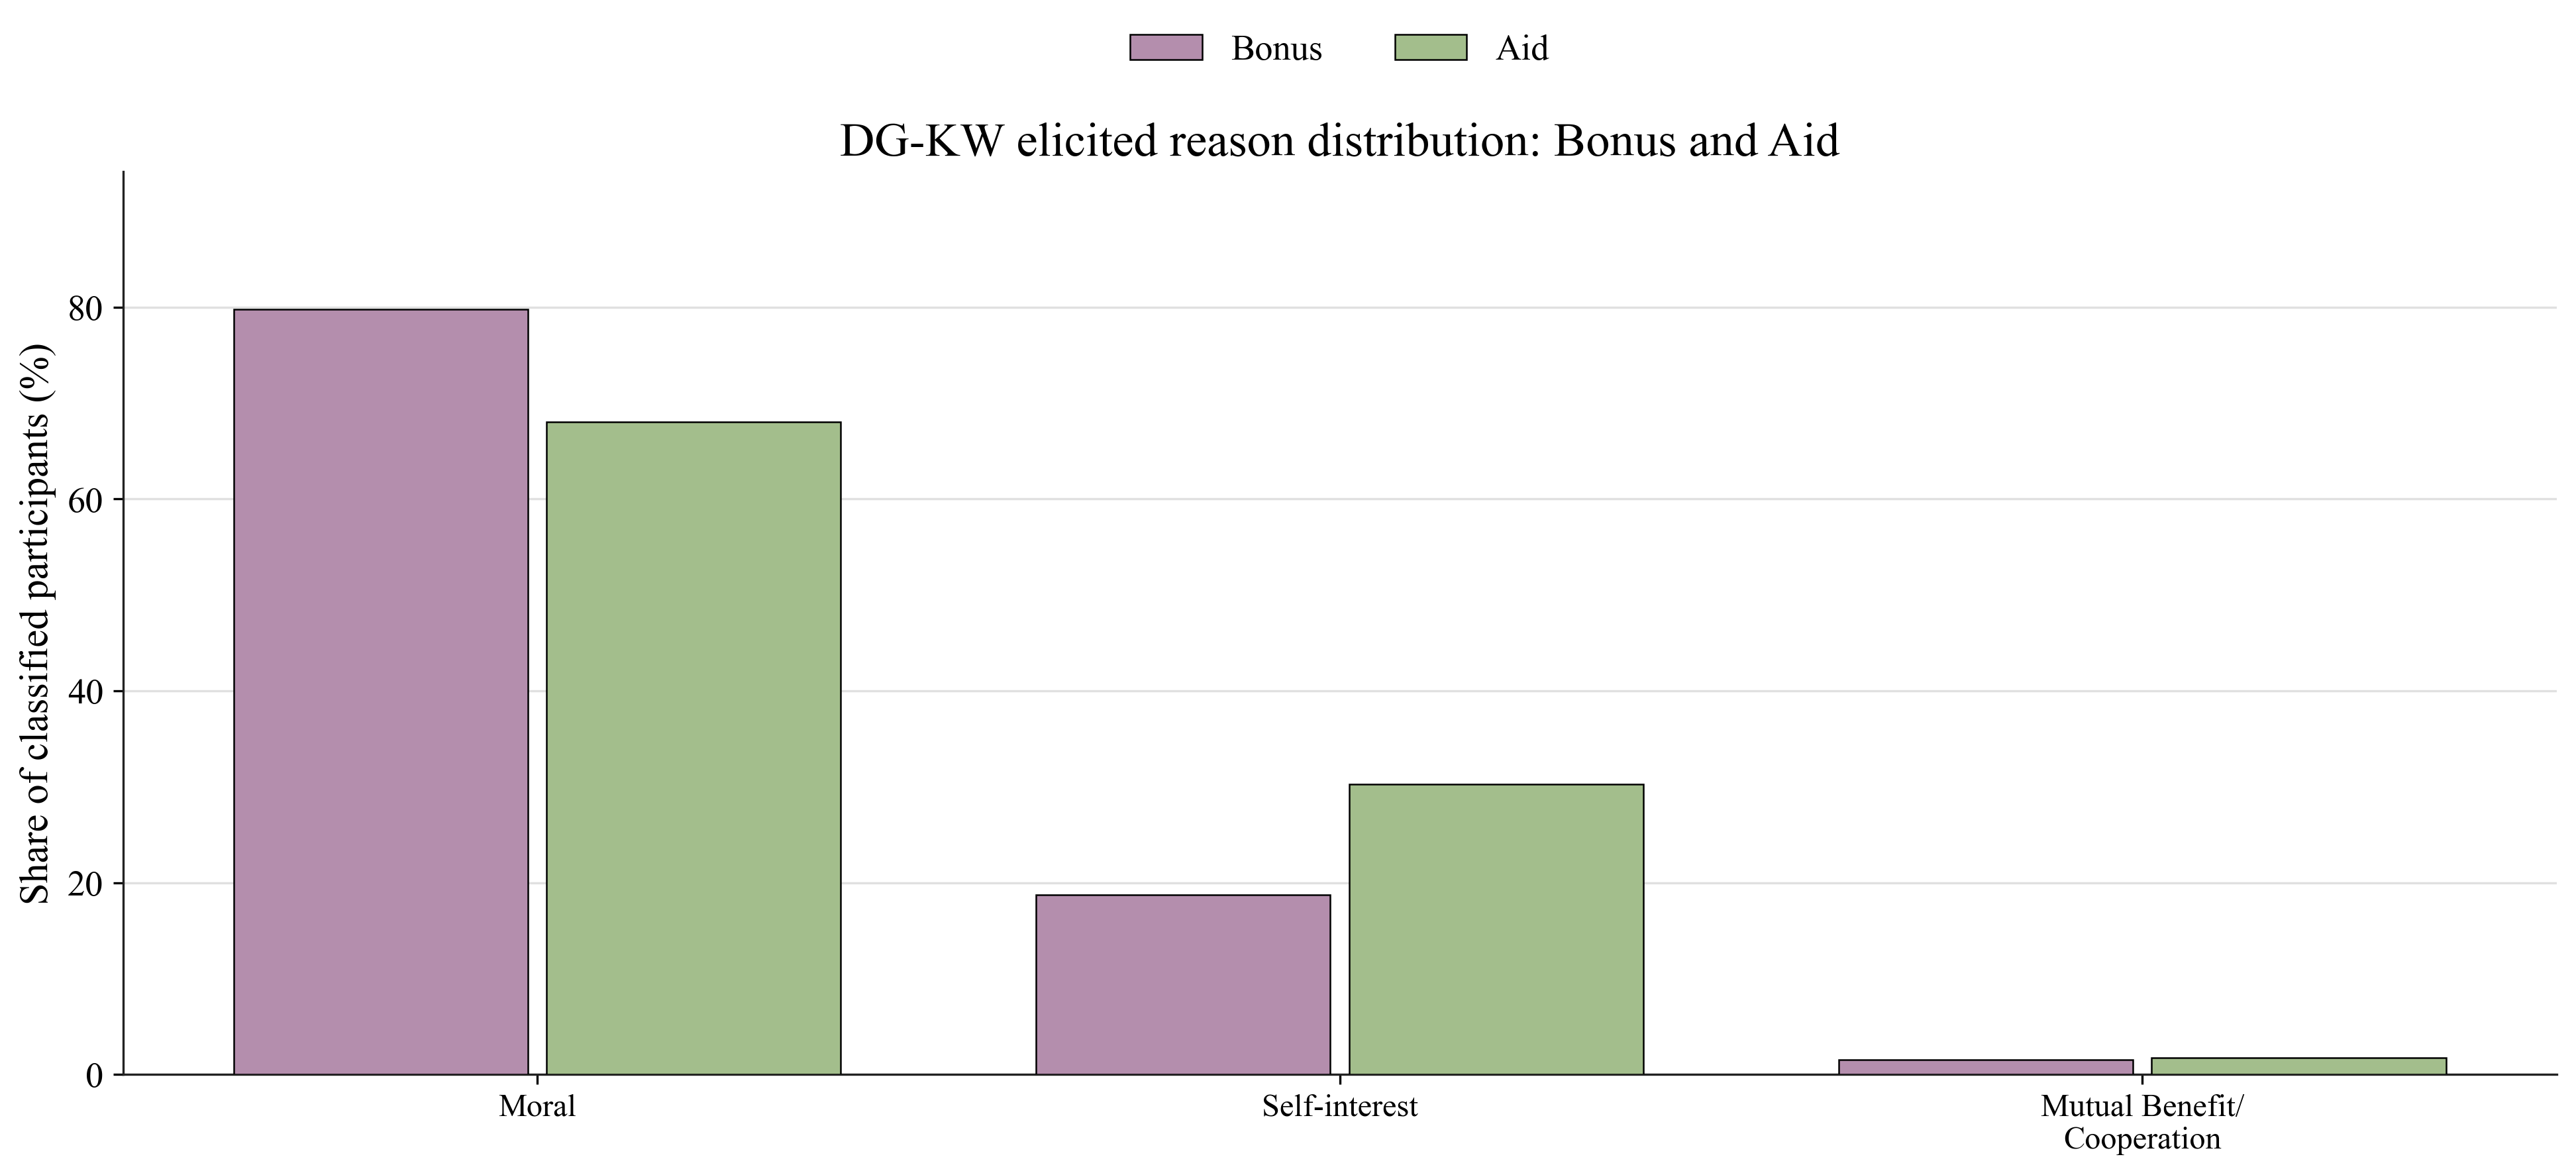
\includegraphics[width=0.95\textwidth]{elicited_dg_bonus_aid_category_distribution.png}
    \caption{DG-KW elicited reason-category distributions in Bonus and Aid}
    \label{fig:elicited_dg_bonus_aid_category_distributions}
\end{figure}

\begin{figure}[H]
    \centering
    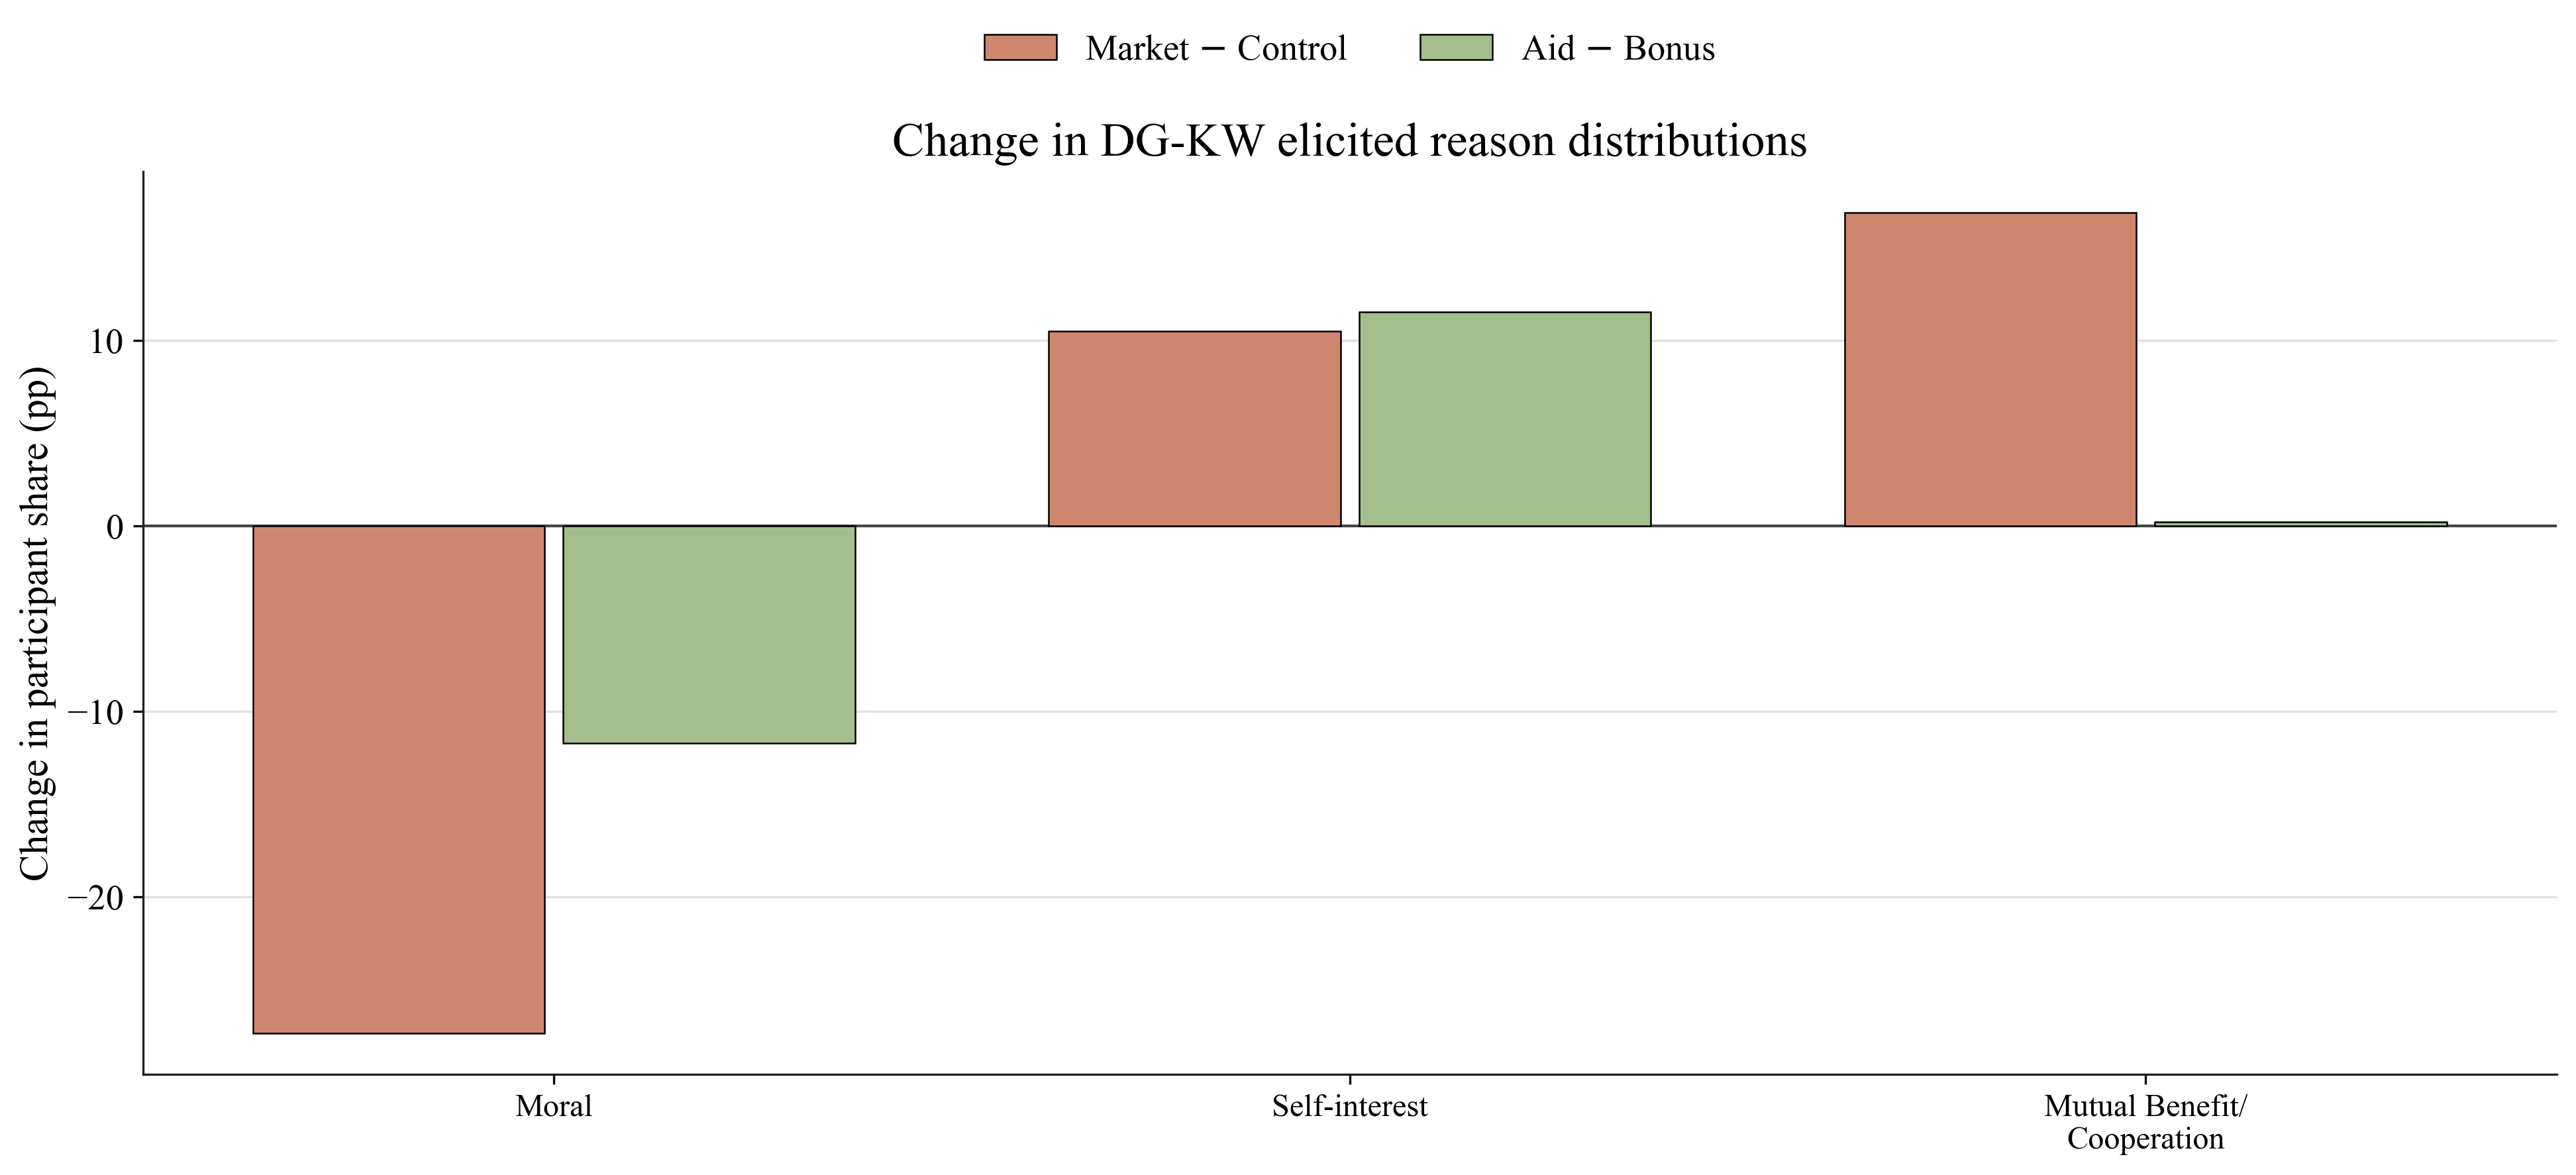
\includegraphics[width=0.95\textwidth]{elicited_dg_category_distribution_differences.png}
    \caption{Changes in DG-KW elicited reason-category shares}
    \label{fig:elicited_dg_category_distribution_differences}
\end{figure}

\end{document}
